\documentclass[12pt,letterpaper]{article}
\usepackage[left=2.6cm,top=2.5cm,right=2.6cm,bottom=2.5cm]{geometry} 
\usepackage[english]{babel}
\usepackage[utf8x]{inputenc}
\usepackage{amsmath}
\usepackage{eqnarray}
\usepackage{mathtools}
\usepackage{tikz}
\usepackage{amssymb} 
\usepackage[retainorgcmds]{IEEEtrantools}
\usepackage{booktabs,caption}
\usepackage[flushleft]{threeparttable}
\usepackage{graphicx}
\usepackage{caption}
\usepackage{tabularx}
\usepackage{subfig}
\usepackage{kpfonts}    % for nice fonts
\usepackage{microtype} 
\usepackage{booktabs}   % for nice tables
\usepackage{bm}         % for bold math
\usepackage{listings}   % for inserting code
\usepackage{verbatim}   % useful for program listings
\usepackage{color}  
%\usepackage[colorlinks=true]{hyperref}%%TABLE % use for hypertext
\usepackage[colorlinks = true,
            linkcolor = blue,
            urlcolor  = blue,
            citecolor = blue,
            anchorcolor = black]{hyperref}
\usepackage[colorinlistoftodos]{todonotes}
\usepackage{natbib}
\renewcommand{\baselinestretch}{1.25}
\setlength{\parindent}{0.5cm}
%\setlength{\parskip}{\baselineskip} 



\begin{document}

%+Title
\title{\LARGE{The effect of house prices on long term care market: Evidence from England}}
\author{Eduardo Gonzalo Almorox\thanks{Newcastle University Business School. 5 Barrack Rd, Newcastle upon Tyne NE1 4SE} \thanks{Corresponding author: \tt{e.gonzalo-almorox@newcastle.ac.uk} } \and Nils Braakmaann\footnotemark[1]
 \and Volodymyr Bilotkach\footnotemark[1] \and John Wildman\footnotemark[1]}


\date{First version: January 2017\\ This version: April 2017}
\maketitle

\begin{abstract}
This paper investigates how house prices affect the market of care homes in 
England. Local markets where the house prices are high may disincentive the establishment of care homes 
and suppose a restriction in the access to long term care services. Alternatively, 
 those markets with high prices may also suppose a business opportunity with a greater proportion of wealthier clients willing to 
 pay more for long term care services. Considering the variation of the planning regulations accross 
 local authorities authorities for addressing
 potential endogeneity in the house prices, our instrumental variables estimates suggest that higher house prices lead to a reduction of 
 the distribution of care homes. Further analyses explore several possible mechanisms driving 
 our results. 

\end{abstract}

{{\bf{Keywords}}: Care homes, house prices, long-term care, England\\
\bf{JEL}: R31, I12}

%\newpage
%\tableofcontents
%\newpage
%-Title


\newpage
\section{Introduction}
\label{sec: intro}


During the last decades, the English housing sector has experienced
 the fastest growth in prices amongst all OECD countries. This growth has been 
 characterised by a high degree of fluctuation. 
 These trends have had consequences in the society
  for both households, notably materialised in the so called
   “house affordability crisis”, and to less extent businesses. 
   In this paper we investigate the effects
    of these price increases on the market structure 
    of an industry that typically operates with low margins,
     the care homes that provide residential long term care services.
      Our interest in the long term care is not trivial.
       Elements such as the ageing of
        the population\footnote{Over the period of 2001 and 2011,
         the proportion of people over 85 has grown faster than the
          population as whole. Apart from living longer,
           this group of population is also more likely to have
             care needs \citep{nao2014}} or some socioeconomic 
             changes such as the the inclusion of more
              women in the labour force or family 
              structures with less members, are shifting the supply
               from the unpaid informal caregiving towards more formal long
                term care provision\footnote{There is mixed evidence concerning the degree
                 of substituability and complementarity between both types of long term care provision 
                 \citep{van2008informal, bolin2008informal}}. These patterns evidence the importance of this sector in the forthcoming decades.
                  Yet, despite the will of policy makers to design policies that preserve
                   a sustainable provision of long term care and that also ensure competitive
                    market structures, there is limited evidence for the design of these policies. 
                    In this paper we aim at informing these policies by analysing the effect of
                     high house prices on the entry pattern in the market of care homes. 

The way high prices in the housing market may affect the local long term care markets is   \textit{a priori} 
uncertain, as there are two opposing effects that may appear. The first may consist of the effect of house price 
as a cost for running a care home. Hence, higher house prices may suppose an important barrier that can restrict the
 entry in certain local markets. Furthermore, higher house prices may increase the opportunity costs of alternative
 building projects and therefore provide an incentive to deter potential development of care homes.\footnote{Some
 representatives of the sector argue that care home developers would  be `` \textit{financially driven rather than 
 reflecting the regional demand}'' \citep{corbett2015}} 
 A potential consequence derived from the former situations could be that people living in
  these areas may find lower long term care choices closer to them. 
   
  A more subtle effect is related to how house prices may affect the demand 
  of long term care. In general, higher house prices reflect a greater level of
  quality in the area (Ross and Yinger, 1999) and are also associated with 
 more economic opportunities \citep{ratcliffe2015wealth}. Besides, housing 
 represents an important part of the household portfolio and then the formation 
of wealth among households is directly linked to the evolution of house prices \citep{rosenthal2004evidence}. In the case of the potential clients of long term care, such as old homeowners, there is mixed evidence on
how the house prices affect their wealth portfolio. Some authors argue that house prices are negatively affected by aged populations (see for example \citet{mankiw1989baby} or \citet{takats2010ageing}). The 
main argument is that people in younger ages are likely to have greater demand. 
Alternatively, houses can be considered as durable capital goods that could 
be monetized by old homeowners by selling them and moving out to cheaper areas \citep{hilber2016housingpolicies, hiller2016aging}. 
Previous literature on long term care markets has considered the level of prices 
in the housing markets as a good indicator of the payer composition 
\citet{darton2010slicing}.

If the former argument holds, areas with higher 
     prices may be associated with greater levels of affluence and consequently greater proportions of clients
      that are more willing to pay for the services of a care home. Although the latter may contribute to preserve 
      the financial viability of care homes in the market (an issue that constitutes a current public policy concern) 
      and also incentivise their entry in these markets, it may also result in an unequal distribution of long term care across different areas in England. 
       In this case, most affluent areas would be more benefited from a greater supply of home care services. 


The main result of the paper is the negative effect that high house prices on the distribution of care homes. 
 This effect suggest that a one standard deviation 
increase in the house prices, reduces the number of care homes per old population from about 0.2 to about 0. 4 depending on the instrument used.
These results suggest that the providers' decision is mainly driven by elements that determine 
the supply of the service and show evidence another social cost associated with the increases of the prices in the housing markets
in England.  

To obtain our results, we construct a dataset that merges information from several sources regarding the characteristics 
of the dynamics in the care homes market, the housing and the long term care markets and the planning regulations. 
Our dataset captures information regarding local authorities 
 at different level (e.g. street, district and county level). A technical hurdle concerning our empirical analysis is 
 linked to effect of house price on care homes entries. For example, it may be possible that the decision of care home providers 
 for selecting certain markets where there are high house prices is driven by unobservable variables
  that make this decision non-random. This sample selection bias may invalidate the estimates corresponding
    to the effects of house prices. In order to overcome these, we carry out and identification strategy which 
    uses an instrumental variables approach that exploits the variability in the restrictiveness of planning
     regulations across English districts. Our identification relies on the assumption that changes in the planning
      requirements affect the entry of care homes in market through the levels of house prices. 

      
This paper contributes to the growing literature on the study of the residential long term 
care market in England. To the best of our knowledge, it is the first that provides causal evidence with
 regards to the effect of housing prices on the context of entries in the market of care 
 homes. Yet, there are several  papers close to the framework where this paper lands. \citet{forder2014}, provide
 a detailed analysis of elements that determine the competition 
 amongst care homes and assess the 
  consequences of this competition in both prices and quality. Other authors, have explored the dynamics of the market
  by analysing potential elements that may lead to care homes closures. \citet{netten2003, netten2005care} find that prices have 
  a negative relationship with closures and \citet{allan2015} investigate the effect of other effects such as the quality or the degree 
  of competition. Their main result suggests that poorer quality and more competitive markets are elements that increase
  the probability of exit from the market.   
 
 We extend this literature by addressing issues referred to the entry process of care homes in local markets. 
  Prior to this paper, only \cite{machin2002minimum} have provided some empirical evidence of factors affecting the market
   entry in the context of a minimum wage regulation. Their results suggest that the introduction of the minimum wage
   affects negatively the entry of care homes; although this effect seem to be not significant.
   In addition to providing a more up to date
    evidence, this research uses a more extensive dataset provided by the regulator, the
     Care Quality Commission (CQC). Likewise, this research also extends the literature that studies the effects 
     of the planning system and the high house prices in England using the care homes as a sector
      for the analysis. 
      
      This paper is organised as follows. Next section, section \ref{sec: institutional}, outlines the 
      main institutional characteristics of the English local government. Section \ref{sec:data} describes  the 
      data used for the analysis and section \ref{sec: empirical strategy} presents the econometric model 
      and the empirical strategy to address potential empirical concerns. 
      Section \ref{sec: results} discusses the results and section \ref{sec: conclusion} 
      concludes.
      
  \section{The institutional setting}
  \label{sec: institutional}
\subsection{English local government}

In England, activities such as the urban planning or the long term care are activities which are responsibility 
of local governments. These are structured and organised according to 
two main operational systems, one tier or two tier, and are associated with different types of local 
authorities. On the one hand, two tier systems have thee county councils, which are the upper tier and cover wider 
geographical areas, and the district councils that constitute the lower tier and comprise 
more local geograhical areas. In these \textit{two tiers}, both county and 
district councils are in charge of different types of activities which in some cases overlap.  

On the other hand, \textit{one tier} systems involve unitary authorities. These 
are local authorities that are in 
charge of the provision of all the activities at local level. Besides, unitary authorities may have two special subcategories
that include the metropolitan boroughs and London boroughs.\footnote{There is another \textit{tier} in some areas of England that
includes town and parish councils which rule smaller local services.}

Taking into account the former main categories, England has a total of 353 local authorities that include 27 
county councils, 201 district councils and 125 unitary authorities. 

 \normalsize{\subsection{Long term care}}
 
 Long term care is managed 152 local authorities that operate at council level.\footnote{Before 2008, these activities
 were managed by  Primare Care Trusts (PCT). The Health and Social Care Act (2008) 
transfered public health matters from these PCT to local authorities. Other issues where PCT were responsible for, such as clinical and health issues, 
became responsibility of the clinical commissioning groups (CCG).} 
These responsibilities over long term care entail mainly the commissioning – i.e. purchase of services 
for those clients who are eligible for public support.  Since the mid-eighties, market mechanisms have driven the provision of long term care services 
both for residential and nursing care. As a consequence, the \textit{for profit} private sector has emerged as the  
main provider. Over the period of three decades from 1984 to 2014, the share of 
private places in England as well as other parts of the UK,  increased a 198\%  being in 2014 a 74\% of the total places. 
This increase was at the expense of public places which decreased a 84\% and supposed a 8\% of the available places 
in 2014. The remaining 18\% of the places were provided by the voluntary sector \citet{jarret2017}. 

There are 19 private and 6 voluntary providers that own about a 30\% of the beds available. Within these, 
4 “main providers” are big chains that concentrate a 15\% of the market share. 
This issue, which implies an increase of the care homes that are owned by the same provider and therefore
a reduction of the competition, has not received much attention in the studies analysing the competition in
the nursing or care homes market. An exception considering the American nursing homes market  
is \citet{hirth2017effects} who find differences in the level of concentration 
in the market when accounting for common ownership.  However, given that these results concern 
only a 20\% of the markets considered, authors suggest that the startegy of the care homes chains could 
be more focused on expanding over new markets.  The remaining 70\% of the market share is composed by providers 
  that have a reduced number of beds - no more than 0.4\% of the beds each.  Despite 
  being very fragmented, the market for care homes presents a high level of competitiveness 
  overall which is not evenly distributed accross the different local authorities \citep{forder2011, forder2014}.\footnote{Considering registered
    care homes in all sectors, the South East is the region that has more
     registered care homes (currently more than 1,000). This proportion
      of care homes contrasts with the North East where there are about 360 registered care homes.}
 
  These regional divergences are explained in great extent by the type of clients that demand 
  residential long term care services in each local authority. Generally speaking, 
  there are two types of clients depending on how their services are funded. Hence, 
 private \textit{self-funded} clients purchase their care 
 according to market rules and their willingness to pay for different types of 
 services. Alternatively, there is also a proportion of clients who 
 undertake a means test in order to determine 
 their eligibility for public support. In the case of this type of clients, the sector works as a quasi 
 market.\footnote{As introduced by \citet{legrand1991quasi} in these markets the 
 state is not the funder and the provider of the services; rather, it becomes 
 a funder that purchases services from a set of private providers that compete 
 against each other. \citet{barron2017quasi} analyse the performance of different types of providers in these 
 markets.}. The proportion of publicly funded is notably more than self-funded clients.\footnote{Using information
  from Laing Buisson market reports, \citet{jarret2017} argue that publicly 
  funded clients would be about a 50\% more than private  clients in 2014.}.

The fact that local authorities have to purchase care on behalf of a significant 
part of the demand, suggests that they may have certain buyer power when negotiating 
the fees applied to public funded clients. A consequence of the former is the 
potential cross subidisation of privately funded clients in favour of the publicly 
supported who would face more reduced fees for the same service. These differences in price 
have
been documented both in the English long term care market \citep{oft2005, hancock2010, forder2014} 
and in the US \citep{mukamel2002competitive, grabowski2004longitudinal}. 


\subsection{Urban planning}

Unlike social care activities, planning systems are managed at the district level by the local planning authorities. 
 These authorities establish various strategic priorities for the areas, including the fulfilment of 
 local needs at socio-economic, 
  cultural, security and health level. These priorities are set out in the National Planning Framework - a national
  framework aimed at guiding policies that entail development decisions for meeting local needs. 
    The health and social care are issues explicitly addressed by this framework. Concretely planning policies should enhance the collaboration between local planning authorities, 
     public health authorities, commissioners and providers in order to promote healthy communities 
     and analyse the implications of the development of health and social care infrastructures. 
     
   Several authors have investigated the effects associated with the design of the planning system in England 
and the net effects of the land use regulation. The main conclusions derived from this research are essentially
 two. Firstly, planning regulations in England are generally more restrictive than similar regulations in other
  countries \citep{cheshire2009, hilber2015}. Secondly, the level of regulatory tightness differs notably across
 English local governments. Thus, local planning authorities
             in more affluent areas (specially areas located in the South East England) 
                 tend to be more restrictive. A determinant of this heterogeneity 
                 is the different incentives that owners have depending on whether the land is developed or not. 
                  \citet{hilber2013origins} 
                 formalise this idea proposing a model where owners of 
                 developed areas would be prone to promote tigther regulations since they would suppose an 
     increase in the value of their land whereas for owners in less developed area it would be a cost. 
     This greater capitalization effect in more restricted areas would suppose an incentive to landlords and homeowners 
      to promote more limits in local development \citep{hilber2015, hilber2016housingpolicies}. An important consequence
       derived from these tight restrictions has been the substantial 
                  increase of the house prices. Figure \ref{fig: corr_prices_refusal} 
                  illustrates this positive relationship between the house 
                  prices and the historical rate of refusal of major projects. 
                  
               {\centering [INSERT FIGURE \ref{fig: corr_prices_refusal} HERE ]}
                  
                  Likewise, the growth in house prices has been uneven across 
                  different regions in England. As Figure \ref{fig: house_prices} 
                  reveals, areas located in the South East, East and South 
                  West, in addition to London, have registered the higher 
                  increases.  
                  
                                 {\centering [INSERT FIGURE \ref{fig: house_prices} HERE ]}
     
     
   
  
  \section{Data}
  \label{sec:data}
  
 
The data corresponding to  the sample of analysis in this paper cover years from 2011 to 2016 
  that we divide into three time intervals $t  (t = 1, 2, 3)$ that include March 2011 – March 2013, 
  March 2013 – March 2015 and March 2015 – September 2016. These data are 
  retrieved from several sources and are referred to 315 local authorities that operate at district level. We 
  use this unit of analysis because as we have outlined in previous section, local authorities at this 
  level decide on urban planning policies and thus indirectly on the level of prices in the area. 
 
   Our main goal is studying the effect of prices on entry of care 
   homes in the local market. In the spirit of \citet{tokunaga2013factors}, who analyse
 the entry in local markets by private for profit long term care providers in Japan, we use a similar variable to 
 reflect providers' choice. In particular, we use the number
  of care homes per 1000 population that
 are aged 65 or over in the local authority,  as the dependent variable in our model. 
 
 \subsection{Care homes} 
 
 We obtain the information concerning the characteristics and dynamics of the
care homes from the Care Quality Commission (CQC) directory of active and inactive
care homes\footnote{This dataset is maintained by the CQC Directorate of Data and Statistics and available upon request.}
This dataset contains all the registrations of care homes that have carried out a regulated activity since
   2010. The initial sample includes 24,354 records. Our analysis is restricted to the entries from March
    2011 onwards since a substantive proportion of the total registrations (16,054) were 
     carried out during 2010 and the first two months of 2011 as a result 
     of a new regulation.\footnote{Since October 2010 registration in Care Quality Commission  became a legal requirement for every long 
     term care provider wishing to carry out a regulated activity.} As we illustrate in Figure \ref{fig: registrations}, this process 
     was prolonged for the remaining months of 2011, particularly until July. The forthcoming years presented  
     progressively less intense level of registrations.
     
    {\centering [INSERT FIGURE {\ref{fig: registrations}} HERE]}
     
A major strength of this dataset for the purposes of our research consists of the opportunity 
to track the entries and exits of the care homes in the market. Besides, it provides further
 individual information regarding the care homes, that includes 
the number of beds in the care home, the identifier code, the name of the care home, the postcode and postal 
address, the city and region where the care home is located as well as the local authority that a council level is responsible for the 
social care services corresponding to the location of the care home. Likewise, with the exception of the number of
 beds, the same information is available with regards to the 10,750 providers where the care homes of our sample 
 belong to. Given that we do not have any further information available, we assume that care homes 
choose and stay in a market since the date of their registration. 
Analogously, we consider that a care home exits the market in the date that it is deregistered.

Considering the former, a general approach to calculate the proportion of care homes
 that are in the market consists of comparing the identification codes and dates of
  registration and deregistration. Then we can count the number of care homes that
   effectively remain during each period of time. However, given the characteristics of this
    administrative data from CQC it is necessary to stress an analytical caveat associated 
    with the measurement of entries in the market. Concretely, it is important to differentiate 
    those entries that correspond to \textit{ de novo } entrants –i.e. entries corresponding to 
    care homes that effectively produce a new activity, from those that may be spurious referred to incumbent
      care homes that merely change their identification code because of 
      issues such as changes in the address or take overs from a different provider. 
      This matter is frequently found in analyses that use data referred to firm
      registers. Neglecting it, apart from introducing measurement errors potentially,
       may lead to incorrect conclusions regarding the market dynamics and 
      the performance of the firm. \citet{geurts2016firm}, for instance, analyse the effect of this measurement
          problem on the estimations of the firm’s growth after the entry in the market.

For distinguishing \textit{de novo} entries we firstly identify those postcodes
 that are repeated given that they may potentially contain spurious entries.
  Then, we compare the dates of registration, the identification code and
   the number of beds corresponding to each observation (care home)
    in order to identify those observations that effectively can be classified 
    as a new entry in the market. Analogously, we follow a similar process
     for calculating the definite exits in the market.  Concretely, 
     after casting those care homes with duplicated postcodes that
      report a date of deregistration , we compare identification
       codes and number of beds to define the last date as a
        definite exit. Considering the former we can calculate 
        the cumulative number of care homes for each wave and 
        calculate the proportion of care homes for each 1000 inhabitants older than 65.   

      
In the second stage of our analysis we use information
corresponding to quality ratings derived from the system
implemented by the CQC since 2014. On the basis of five 
dimensions\footnote{These dimensions entail the evaluation of issues related to the safety, the effectivity, 
the level of care and response to people’s needs as well as the management of the services.}, this new approach
  set a systematic method for collecting evidence that enables a more consistent assessment and comparison
   of the care homes’ performance. Services are rated according to four categories: {\it outstanding, good, requires
    improvement or inadequate}. For our analysis we collapse these categories into two: bad (requires improvement 
    and inadequate) and good (outstanding and good). Because the information is only available since October 2014, this part of the analysis considers a different
   timeframe that involves three waves October 2014 - May 2015, May 2015 – February 2016 and 
   February 2016 – September 2016. 
   
%   Likewise we test the effect of the house prices on the level of 
%    residential care expenditure for each local authority. We represent the level
% of public expenditure throughtout the yearly gross current expenditure per adults over 65.\footnote{This is a well established fiscal measure of 
% government spending and it represents the expenditure that is not offset by income from clients and does not include capital charges either. Gross current expenditure $G$
%  is calculated as: $G = T - C$ where $T$ is Gross Total Expenditure and $C$ incorporates capital charges. 
%  Likewise, $T$ is obtained from deducting incomes from joint arrangments $I$, the NHS $N$ and other incomes $O$ to the total expenditure
%   $E$, $T = E - (I+N+O)$} For our analysis we select 
%  information corresponding  to the report of years 2011/12 to 2015/16 released by the NHS Digital\footnote{Further details
%   may be found in \href{https://www.digital.nhs.uk/article/219/What-is-NHS-Digital-}{https://www.digital.nhs.uk/article/219/What-is-NHS-Digital-}} (formerly the HSCIC). 
%   
  \subsection{House prices} 
  
  The information corresponding to prices of the properties is obtained from the price paid dataset
    released on a monthly basis by the Land Registry. This dataset contains all the transactions of
     properties carried out in England and Wales since 1995. In addition to the price paid for the transaction,
    the dataset includes further information such as the type of property, the address, the city, district
     and region where the property is located as well as other information such as whether it is newly built
     and whether the property is under leasehold or freehold\footnote{The difference between these two types properties is based on 
     the whether the ownership of the land or property is for a temporary (\textit{leasehold}) or unrestricted ( \textit{freehold}) period. }. 
     The information regarding the transactions is
     collected on a daily basis and we are able to subset it according to the pre-defined periods of
     analysis. Then we group transactions that belong to the same planning authority and retrieve the average 
     price of them. The final output consists of the average price for each local planning authority for each
    period of analysis. 
        
  \subsection{Urban planning and electoral data}
    Inspired by \citet{hilber2016supply}, our identification strategy exploits changes over time in the restrictiveness of the 
planning regulations. This variable is built considering a series of historical
  planning applications from the Department of Communities and Local Government (DCLG) 
  since 1978 and it is defined as the refusal of projecst that entail 10 dwellings or more per year. 
  As we shall explain in further detail 
    below, this measure may be subject to endogeneity concerns. In order to correct for 
    these potential limitations, we use an alternative measure 
    of planning regulations, the rate in change of delay of major projects which is also obtained from the DCLG. We
    also use the variation in the historical 
    political composition of the local authorities. Using data from the British Election Studies Information System, 
    we capture a series of the historical Labour vote share at the General Election since 1983. 
    In order to control for possible bias of associated with the former, we 
    also include data on the most recent election corresponding to June 2015. 
    Data are obtained from the Parliament website platform.\footnote{Further information is provided 
     in the following link: \href{http://www.data.parliament.uk/dataset/general-election-2015}{http://www.data.parliament.uk/dataset/general-election-2015}}.
     Likewise there are may be other factors that detemine the house prices such as for example the share
     of developable land. Since this variable can suffer from endogeneity, we use the historical population density 
     associated with the developable land. 
    
   \subsection{Local long term care markets}
    
    Finally, our regressions also include a number of control variables 
    that represent various characteristics of the local long term care markets. These variables are retrieved mainly from the Department of 
    Work and Pensions (DWP) and we provide a more detailed justification of 
    their choice in the next subsection.
  
 Table \ref{descriptive_stats} shows descriptive statistics of the 
 main variables in our sample.The information is presented at the district level. 
 
 
  {\centering [INSERT TABLE \ref{descriptive_stats} HERE]}
 
 On average, over the period of analysis
 there were about 1.7 care homes per 1000 population over 65. 
 Yet,  this proportion varied notably across the different local authorities 
 where some present less than 1 (0.4) care homes per 1000 population
  and some others more than 3.5 up to a maximum of 4.06. Figure \ref{fig: map care homes} plots the spatial distribution
  of care homes. In general, neighbouring districts present a similiar 
  distribution of care homes per old population. There are some exceptions corresponding to some districts in the 
  North West and Central North where the distribution of care homes is between 2 and 4 care homes per 1000 people over 65.\footnote{These districts
  are Allerdale, Lancaster, Harrogate and Scarborough.} 
  The southern districts (i.e. South West and South East regions) have the 
  greater amount of care homes per old population. 
 
 
  {\centering [INSERT FIGURE {\ref{fig: map care homes}} HERE]}
  
  
 Other variables of interest in Table \ref{descriptive_stats}
  also reflect geographical variation although the picture is more homogeneous than in the case of the geographical
  distribution of care homes. Figure \ref{fig: map house price} 
  discovers the distribution of house prices across the English districts. There 
  is a clear dichotomy between local authorities situated in the north and in 
  the south of country. Also, there some extreme cases of local authorities where the 
  average value in the properties registers a maximum £2,170,757. Apart from this outliers, the average house price
  of the sample is £268,764.
  
    {\centering [INSERT FIGURE {\ref{fig: map house price}} HERE]}
 
 \section{Empirical strategy}
 \label{sec: empirical strategy}
 
 The purpose of our analysis is to study empirically the effects of the house prices on the proportion of care homes in local
  long term care markets. The main analysis is based on regressions that model 
 the distribution of care homes in a reduced form as follows
  
%   \begin{eqnarray}
%      C_{it} =\alpha P_{it} + \epsilon_{it} \label{naive}\\
%      
%      C_{it} =\beta X_{it} + \alpha P_{it} + \epsilon_{it}
% \end{eqnarray}
 
 \begin{equation}
  \label{equation: carehomes_prices}
  \begin{aligned}
    C_{it} =\alpha P_{it} + \epsilon_{it} \\
    C_{it} =\beta X_{it} + \alpha P_{it} + \epsilon_{it}      
  \end{aligned}
\end{equation}



The first expression in Equation (\ref{equation: carehomes_prices}) refers to the raw correlation between the
 proportion of care homes per 1000 population over 65,  $C$, in a local authority $i$ in a time period $t$ 
 and the average of the house prices, $P_{it}$. $\epsilon$ represents an error term that is identically and independtly distributed. 
The second expression adds some basic exogenous control variables that 
characterized the composition of the long term care markets and are gathered in 
$X_{it}$.  Specifically, we include the proportion 
  of people older than 85 and proportion of people that receive the attendance 
  allowance\footnote{This benefit aims to support those people with physical disabilities in UK that live
   independently and might require residential care services otherwise. } as proxies of the level 
   of health dependency. Also, given the association between the financial needs and the funding
    support determined by the means-test, we incorporate the proportion of people that receive some
     sort of income support and the proportion of people that receive pension credits to reflect the payer 
     composition within the local population. These variables have been previously used in the literature for these purposes 
     \citep{darton2010slicing, forder2014}. Likewise, given that long term care is a labour intense 
     activity and it is specially carried out by females\footnote{This proportion is about 82\% in 2016 \citep{workforce2016}}
      we add the proportion of females that claim for job seekers’ allowance in order to get a proxy for 
      unemployment. In addition to the former, we also include in $X$ a measure of the Herfindahl–Hirschman Index (HHI) to control for
      the competition between care homes in the local market. In our case, the HHI is a measure of concentration that 
      reflects the squared shares of beds across all the providers in a local market. The values range from
       0 to 1 where higher values represent higher concentration and therefore less competition.  
 
Equation \ref{equation: carehomes_prices} can be estimated by OLS and the parameter of interest, $\alpha$,  may be interpreted as a causal effect
  of the house prices on the distribution of care homes, only if
         $P_i$ is exogenous so that $Cov(P_{i}$,$\epsilon_{i}) = 0 $. 
         Nonetheless, the entry of a care home in a particular local long term 
         care market may be determined by additional factors other than house 
         prices that scape to the control of observable variables. If the 
         influence of these potential unobservable shocks is not appropriately 
         undertaken, the OLS estimations of $\alpha$ may be inconsistent. 
         
  An example that may illustrate the latter could be an unobserved shock that may affect positively the values of the properties and also incentivise
   the entries in the market given likely wealth effects. Hence, higher level of housing prices may result in
    wealth effects that lead to greater levels of consumption and then attract businesses. This implies that the selection
     of an area by a care home provider is likely to be \textit{known} -non-random,  and the effect of $P_{i}$ may be associated partially 
     with $\epsilon$. Likewise another potential problem may arise on the basis 
     that, in addition of $C_{i}$ being determined by $P_{i}$, $P_{i}$ also could be determined partially as 
     a function of $C_{i}$
     
     In order to tackle with these problems associated with $P_{it}$, we consider an instrumental variables (IV) approach, 
     where we use an instrumental variable $z$  that is uncorrelated with $\epsilon$ but is correlated
       with $P_{i}$. Inspired by \citet{hilber2016supply} our identification 
       strategy exploits the restrictiveness in the local planning regulations. 
       \citet{hilber2016supply} use this variability for analysing the effects of local earnings
 on house prices. Their findings confirm the vision that tight supply regimes – e.g. with more regulatory 
 constraints in the planning regulations, lead to increases in the prices. In our case, however, we apply 
the planning regulation variable as direct instrument to the house prices. For our identification we assume that this instrument,
  in addition to being correlated with the local earnings, is also correlated with the house prices. The measure that we use is the 
 rate of refusal of major projects. It is normally used in the literature and 
 reflects the share of applications corresponding to projects that entail 10 or more 
 dwellings that are rejected by a local authority during a year.  
 
 Both the relationship between
  planning regulations and house prices as well as the use of planning regulations 
  for addressing endogeneity bias associated with house prices have been well documented in the literature. 
  Considering the case of UK for instance, several authors have shed light with regards to the effects of tight planning 
  regulations on house prices suggesting a positive relationship \citep{cheshire2009, cheshire2014, barker2004barker, hilber2016supply}.
  A potential problem with this instrument is that is procyclical and this may 
be introduce bias. For example, developers may modify the way they apply when they are aware of the level
 of tightness of certain local planning authorities are tighter than others. It may happen that if they know
  that some local planning authorities are particularly restrictive they may withdraw their applications and focus
   on other markets. If this occurs, then the observed refusal rates may not reflect the level of real 
   restrictiveness, especially in the cases of more limiting local planning authorities. 
 For coping with this limitation it is possible to exploit two identification strategies on the basis of \citet{hilber2016supply}.
    
    The first involves a planning reform aimed at speeding up the planning processes and the
   second links the planning regulations and the variation in the share of local political power. 
The main idea corresponding to the identification strategy based on the planning reform consists
 of exploiting the variation in the change in the delay rates before and after the reform. Set in 2002,
  the reform included the establishment of an explicit goal for major development projects. The main
   purpose of this target was to avoid the delays of major projects by local planning authorities. 
   Even though they were not formally penalised for not meeting the target, local planning authorities did not have
     the incentive for neglecting the target either. The central government could retain financial resources
      addressed to local planning authorities. An option for local authorities to meet the target was to refuse 
      greater projects and conversely approve smaller projects which could be finished on time. 
      
On the basis of the former, it is possible to think on the behaviour of the local planning authorities
 before and after the reform paying particular attention to their level of restrictiveness. Thus, before 
 the reform local planning authorities that were more restrictive would be also the ones that had greater 
 delays and thereby the least likely to meet the target. Once the reform was established, these local 
 planning authorities would be also the ones more likely to refuse more projects and therefore suffer less
  delays. Less restrictive local planning would not have to alter their behaviour substantially.
   Considering this, we allow for a 10-year period to represent the average delay rates pre and post reform.
    Hence we consider the delay rates 1994 and 1996 and the delay rates between 2004-2006.  
    
The alternative strategy consists of taking advantage of the relationship between the political composition of local councils
 and the application of local planning regulations. In addition to 
 \citet{hilber2016supply},
  similar strategies have been used by other authors such \cite{bertrand2002does} or 
  \cite{sadun2015}. 
  Hence, we use the share of Labour party votes at the General Election of 1983.
   The information is obtained from the British Election Studies Information System.  
   We choose the share of Labour voters since the attitudes of these voters 
   regarding construction
   will be more on the basis of the job implications and inclined to grant house access rather than to preserve
    the value of the properties \citep{cheshire2016}.
    Also, we could have used the results derived from local elections. 
    Yet, these might be correlated with the development of local housing markets and constitute a source
     of potential bias. The time frame of 1983 provides the earliest date where election results can be linked
      to data corresponding to local authorities and then minimizes the potential association between the
       outcome of the election and the planning process.



In addition to the planning regulations, there may be other drivers that entail 
restrictions in the supply of houses and thus may lead to increases in the house 
prices. Physical constraints may be an example of those and should be included in the 
estimation. We use the share of developed land to express the extent of physical 
constraints. A potential limitation referred to this variable is that 
  the availability (or scarcity) of this type of land can be the result of elements that 
  also affect the house prices and therefore may imply endogeneity. For 
  addressing this problem, the historic population density can be used as an 
  instrument for identifying the share of developable land since it may show the 
  early forms of agglomeration. We use the historic population density in 1911 
  as an instrument for the share of developable land. 
  
Considering these caveats, we specify Eq. (\ref{equation: firststage_prices}) in order to estimate the
 first-stage fitted values of the
 house prices. The predicted values derived from this equation are used then as instruments and incorporated in
 Eq. (\ref{equation: carehomes_prices}) in order to get a consistent estimate of $\alpha$

  \begin{eqnarray}
\label{equation: firststage_prices}
    P_{it} = \delta Z_{it} + \beta \chi_{it} + \eta_{i} + u_{it} 
 \end{eqnarray}

 where $Z$ refers to the variable associated with the planning regulation (e.g. the rate of refusal of major projects) and $\chi$  
 to the variable referred to the physical constraint (e.g. share of developed land). An  In addition to the specification developed by 
\cite{hilber2016supply}, we include $\eta$ as a control for the contemporaneous share 
 of Labour voters for each local authority. The data corresponds to the results at local level of the national election in June 
2015.  As we noted before, a potential issue for the reluctance of the Labour share as an instrument may be related to 
unobserved trends. For instance, some areas have been exposed to the inflow of
certain residents that may changed the demographic composition of certain areas and this also modified the voting behaviour. In order to 
control for this we include the share vote for each local authority 
corresponding to the results of the last national elections celebrated in June 
2015.\footnote{ \citet{cheshire2016} use this instrument for analysing the effect of planning regulations on the 
proportion of vacant houses in England. They provide housing markets in Greater London as an example of areas
that could have changed  their voting behaviour as a consequence of these inflows.}

Furthermore, another difference of our approach in comparison to their empirical strategy from \citet{hilber2016supply}, is that we use two instruments for 
identifying the house prices rather than a single instrument for identifying variables that determine them such as the 
planning regulations and the share of developed land respectively.

Table \ref{table first_stage} shows evidence on the validity of the instruments that we could consider for overcoming 
the endogeneity problems in our analysis. On the basis of the regression
specified in Eq. \ref{equation: firststage_prices}, column (1)
provides the estimates referred to the relationship between the rate of refusal and the 
house prices. The positive relationship between the level of regulatory tightness in the planning 
regulations and house prices is consistent with previous findings shown in the literature. Nonetheless,
 for the reasons exposed above, the 
rate of refusal may suffer from endogeneity so considering the regression with only this instrument
 would invalidate our results corresponding
to the second stage. Columns (2) and (3) present the estimates 
corresponding to the instruments proposed to tackle with this limitation - the 
change in the rate of delay and the local share of Labour voters respectively. 
These results associated with these estimations point at the direction that we would expect. Greater changes
 in the delay rates pre and
 post reform influence negatively the house prices. These big differences would imply 
 greater reductions in the rate of delay for restrictive local authorities which would be substituted with more
  rejections of the major projects and therefore 
  greater refusal rates. Likewise, the share of Labour voters is also associated with lower levels in the house prices. 
Column (4)
includes the estimation results considering only the density in the 
population in 1911 as the single instrument and column (5) include all
former instruments in the regression. 

  {\centering [INSERT TABLE {\ref{table first_stage}} HERE]}


The bottom of Table \ref{table first_stage} shows various tests that assess validity of the instruments. First, we 
evaluate the strength of the correlation between the instruments and $P_{i}$. The join $F$ test of excluded instruments is highly significant at
at a lower level than 0.01 in all the cases. On the same basis, we also present the results of 
weak instruments test using a Cragg Donald Wald $F$ statistic and a 
Kleibergen-Paap Wald rk $F$ statistic. Similarly, the results yielded by these tests suggest
that weak instruments do not seem to be a problemd in our regressions.

Second, since our estimations use in some cases various instrumental variables for identifying a single endogenous variable,  
we present the results of over-identification tests based on 
\citet{sargan1958estimation}\footnote{The statistic resulting from this test is distributed as a $\chi^2$ distribution under
the joint null hypothesis that the instruments are valid instruments.}.  The $p-values$ referred to the 
 statistic considering the rate of refusal and the share of Labour voters (columns (1), (3)  and (5) respectively) are lower than 
 0.01.  This suggests the rejection of the null hypothesis of valid over identification restrictions and 
  raises a caveat when interpreting the results derived from these 
  specifications since not all the instruments may be identifying the the same vector of parameters  
  \citep{parente2012cautionary}.
  


\section{Results}
\label{sec: results}

\subsection{House prices and market entries}

Table \ref{table second_stage} reports the main results derived from the estimation of the impact 
of house prices on the proportion of care homes based on the second stage of our 
specification presented in Eq \ref{equation: carehomes_prices}. 


  {\centering [INSERT TABLE {\ref{table second_stage}} HERE]}

The results reported in column (1)
show the most basic OLS estimates of the relationship between the house prices and the distribution of care homes excluding 
characteristics of the local market. Figure \ref{fig: carehomes_prices} shows graphically this association which is negative and significant
at the 1\% level. Yet, as we show in column (2), when we 
incorporate controls referred to the local characteristics of the long term care market this 
negative effect diminishes and reduces its statistical power. 

  {\centering [INSERT FIGURE {\ref{fig: carehomes_prices}} HERE]}

As discussed in previous section, the estimates from columns (1) and (2) can not be interpreted as
 the causal effect of the house prices
on the distribution of care homes due to potential endogeneity concerns. The 
remaining columns present results referred to various IV estimates using the rate of delay (column 3),
 the share of Labour voters (column 4),  the population density in 1911 (column 5) and all the instruments (column 6) respectively. 
 The coefficients derived from all the estimates suggest that high prices in the 
 housing markets would effectively disuade the entry of care homes. Hence, increases 
  in the house prices lead to significant reductions in the number of care homes. 
 
A potential concern associated with this effect is that it may not be correctly measured. One may argue that 
the decision of entry in the market may be to certain extent lagged. For instance, providers may base their decision of entry 
on historical house prices rather than the current ones. Also, there is another potential 
problem given by the influence that care homes may have in the value of the properties in an area. 
They may suppose and ammenity that future inhabitants may value and thus affect the prices of the 
properties in the area. Thereby using contemporaneous prices may 
cause simultaneity problems. In order to mitigate these potential limitations, in  
Table \ref{table robustness_lag} we present the results of the estimates 
corresponding to the effects 
derived from house prices that are lagged two years. 

  {\centering [INSERT TABLE {\ref{table robustness_lag}} HERE]}

The effects using the lagged prices are along the same lines as the findings presented in 
Table \ref{table second_stage}. We estimates of Hansen J Stastic report corresponding to the estimations with
the share of Labour voters and all the instruments provide evidence to to reject the null hypothesis of  
valid over identification restrictions and again poses caveats with regards to the 
interpretation of the results under these specifications. 


In Tables \ref{table robustness_outliers_bottom} and \ref{table robustness_outliers_ london} we explore the robustness of our results
to various changes in the sample. It is important to note that the 
specifications are based on Eq \ref{equation: carehomes_prices} 
 and Eq \ref{equation: firststage_prices}. Firstly, a plausible concern may be the presence of some outliers in
  the distribution of care homes. In order to overcome the potential influence
  of these observations we remove from the sample those local authorities that have the top and bottom 5\% of the care 
 homes in the market (94 care homes in total). Table \ref{table robustness_outliers_bottom} 
 display the results of these estimates. 
 

   {\centering [INSERT TABLE {\ref{table robustness_outliers_bottom}} HERE]}
 
The results corresponding to the IV estimates (columns (3) to (6)) present 
heterogeneous effects. In the cases using the share of Labour votes and all the 
instruments (columns (4) and (6)), the effect of the house prices on the distribution of care homes is 
positive. Given the value of the Hansen J statistic, it is possible that these 
specifications could be identifying other parameters than the house prices. The 
specifications with the remaining instruments, the change of the delay rate and 
the population density in 1911, provide negative effects. However, these have 
lost their stastistical power. These findings suggest that that our results 
could be driven by the presence of outliers.
 
 Likewise, we also consider a sample without those care homes that are associated with 
 planning authorities in the region of London (96 care homes). As we reflected in figure \ref{fig: house_prices}, the 
 house prices in this region have experienced the greatest increase during the 
 last two decades. The results from this analysis are presented in Table \ref{table robustness_outliers_ london} 
   and are on the same basis 
 as the results in Table \ref{table robustness_outliers_bottom}. Yet the estimates
 derived from the regressions instrumenting with the rate of delay and the population density 
 report greater effects that are significant at less than 5\% level. 
   
      {\centering [INSERT TABLE {\ref{table robustness_outliers_ london}} HERE]}
   


In general, these findings suggest that the decision of entry by long term care providers 
in local markets may respond more to financial incentives that determine the cost of
development than to other factors associated with the long term care issues. The development of
 a care home in an area where the value of alternative uses of land such as housing are high, also entails a high opportunity 
cost. If this argument holds, given the positive relationship between the level of planning 
restrictiveness and value of the properties, more restrictive planning areas would imply higher 
opportunity costs and therefore the negative effects of the prices on the entry 
of care homes should be more pronounced. 

\subsection{Alternative mechanisms}

We explore the former argument by carrying out the analysis in two samples that gather 
local authorities according to their level of restrictiveness in the planning 
decisions. We select each group of planning authorities on the basis of their behaviour before and 
after the reform that imposed particular planning targets. As discussed before, more restrictive authorities would
modify their behaviour regarding applications of major projects and reduce the delays 
of the applications at the expense of more rejections. If this occurs then those 
local authorities that have negative rates of the change of delay would be more 
restrictive. In figures \ref{refusal_restrictive} and \ref{f2} we describe graphically the distributions of refusal 
rates and prices for local authorities depending on 
the change in their rate of delay before and after the reform. 

  {\centering [INSERT FIGURES {\ref{refusal_restrictive}} and \ref{f2} HERE]}

Tables \ref{table no restrictive} and \ref{table restrictive} report the effects of house prices on the 
the care homes depending on whether the local authorities were delaying equally or more 
after the reform (e.g. non restrictive) or less (e.g restrictive). The regressions are again based on the 
baseline specification so that columns (1) and(2) represent OLS estimates and (3) to (6) IV estimates considering the rate of delay, the share of Labour voters 
the population density in 1911 and all the instruments. 

 {\centering [INSERT TABLE {\ref{table no restrictive}} HERE]}\\
  {\centering [INSERT TABLE {\ref{table restrictive}} HERE]}

In more restrictive local authorities we find a negative and significant effect from the prices 
compared to no restrictive local planning authorites. As introduced before, the 
reason behind these findings would be the greater opportunity costs associated 
with the alternative uses of land in this more restrictive planning authorities. 

In addition to the costs, providers could be focusing
 on more affluent areas possibly aiming at securing potential clients that do not rely on public funding 
 arrangements. A reason for this may be the aim of providers for ensuring a 
 level of clientele that helps them to offset the costs not only of entry but 
 also of the existing cross-subsidisation from self-funded to publicly funded clients.  
  \citet{humphries2016social} argue that this strategy would be followed by a number of long term
   care providers in order to preserve their financial viability and overcome the funding 
   crisis. This argument would suggest that areas with a greater proportion of clients that self fund 
   their care should be more attractive for care homes.    
   
Exploring this mechanism would require information on the
   composition of the clientele associated with each care home. Unfortunately, this information is not publicly available. 
   However, a proxy for the composition of the clientele can be derived
  from the quality rating associated with the care homes. It is sensible to think that people who 
  self-fund their care may have more willingness to pay for greater levels of 
  quality. Care homes with an outstanding level of quality are likely to have a 
  greater proportion of clients that self fund their care. 
  
 {\centering [INSERT TABLE {\ref{table quality outstanding}} HERE]}\\
  {\centering [INSERT TABLE {\ref{table quality bad}} HERE]}
  
  Tables \ref{table quality outstanding} and \ref{table quality bad} report the results of the effect of house prices on 
  the distribution of care homes according their level of quality. The IV estimates (columns (3) to (6))
reveal a positive effect of the house prices on the distribution of care homes 
that obtain an outstanding rating. Although these effects are small, possibly because of the 
reduced proportion that this type of care homes represent out of the total, they are significant at less than 0.05 
when instrumenting with the share of Labour voters and all the instruments. 
Regarding the care homes with a bad rating, the effect is also positive and greater, but not 
signifcant for any of the IV estimates. These findings suggest that effectively care 
homes would be addressing their market strategy to those markets where there is 
a higher proportion of potential self-funded clients. 

\section{Conclusion}
\label{sec: conclusion}

Putting things together, these results imply that high prices in the housing markets 
are a social cost and reduce the number of care homes. The findings appear to 
validate the idea that the development of care homes would be driven by 
financial forces and in markets with high house prices, developers would 
prefer more competitive alternative projects. Given the importance of those observations in the extremes of the sample, 
our results should be read as suggestive rather than definitive. A potential 
avenue for further research should consist of exploring the results in these 
local authorities. 

This paper provides evidence of the impact of the English housing market on 
adult long term care. It is the first that does so by tackling explicitly 
with the endogeneity problems associated with the house prices. The availability of information on planning 
regulations offers a unique opportunity to address them. This paper contributes to the literature aimed at studying
 the connection between the housing market and the
 market of long term care activities. These findings may contribute to improve the coordination between local
  authorities  for the design of both planning and social care policies. 



  
\newpage
\bibliographystyle{apalike}
\bibliography{ex1}
%remember to use \citep{} for citation

\newpage

\section{Tables}

\begin{table}[ht]
\centering
\caption{Summary statistics}
\label{descriptive_stats}
\resizebox{\textwidth}{!}{% 
\begin{tabular}{lrrrrr}
  \hline
 & Obs & Mean & Minimum & Maximum & St.Dev \\ 
  \hline
Care homes per 1000 population over 65 & 945 & 1.6678 & 0.4255 & 4.0611 & 0.5416 \\ 
  Average house prices & 945 & 268564 & 91157 & 2170757 & 179558 \\ 
  Share of population 85+& 945 & 0.0025 & 0.0002 & 0.0122 & 0.0016 \\ 
  Share of population receiving Attendance Allowance& 945 & 0.0106 & 0.0043 & 0.0263 & 0.0039 \\ 
  Share of population with pension credits & 945 & 0.0339 & 0.0130 & 0.0705 & 0.0100 \\ 
  Share of female claiming for JSA & 945 & 0.0047 & 0.0007 & 0.0185 & 0.0032 \\ 
  Share of population with income support & 945 & 0.0122 & 0.0028 & 0.0402 & 0.0059 \\ 
  HHI & 945 & 0.0320 & 0.0064 & 0.4873 & 0.0352 \\ 
  Share of Labour voters 2015 & 945 & 0.2810 & 0.0698 & 0.7301 & 0.1448 \\ 
  Rate of refusal major projects & 945 & 0.2563 & 0.0732 & 0.5090 & 0.0879 \\ 
  Rate of delay change & 945 & -0.0376 & -0.6345 & 0.5310 & 0.2197 \\ 
  Historical share of Labour voters  & 945 & 0.1625 & 0.0010 & 0.4103 & 0.0886 \\ 
  Proportion of care homes (bad quality) & 945 & 0.1905 & 0.0000 & 0.6585 & 0.1232 \\ 
 Proportion of care homes (outstanding quality)  & 945 & 0.004095 & 0.0000 & 0.0870  &0.012 \\ 
 Proportion of developed land & 945 & 0.2729 & 0.0090 & 0.9621 & 0.2356 \\ 
 Population density in 1911 & 945 & 774.7089 & 3.2504 & 22028.7969 & 2633.3879 \\ 
   \hline
\end{tabular}}
\end{table}



\newpage

\begin{table}[h!]
\centering
\caption{First stage results - dependent variable average house prices (log)}
\label{table first_stage}
\resizebox{\textwidth}{!}{% 
\begin{tabular}{@{}lcccccccc@{}}
\toprule
                                           & \multicolumn{5}{c}{Average house prices (log)}                       \\ \midrule
                                    & (1) & (2) & (3) & (4) & (5)\\
                                    \hline
                       
Historical rate of refusal of major projects & 3.142***    &             &             &             &             \\
                                             & (0.161)     &             &             &             &             \\
Rate of delay change                         &             & -0.561***   &             &             & -0.322***   \\
                                             &             & (0.0853)    &             &             & (0.0703)    \\
Share of Labour voters                       &             &             & -2.312***   &             & -2.159***   \\
                                             &             &             & (0.341)     &             & (0.327)     \\
Population density 1911                      & 9.64e-05*** & 8.15e-05*** & 0.000103*** & 8.07e-05*** & 0.000102*** \\
                                             & (1.34e-05)  & (1.11e-05)  & (1.25e-05)  & (1.22e-05)  & (1.18e-05)  \\
                                             \hline

Observations                        & 945          & 945          & 945          & 945        & 945             \\ 
Number of local authorities & 315 & 315  &315 & 315 & 315  \\

F(excluded instruments)             & 206.50***    & 47.26***     & 58.04***     & 43.85***    &   53.81***          \\
\hline
Cragg-Donald Wald F statistic       & 641.313      & 192.834      & 392.101      & 261.942      &  288.52         \\
Kleibergen-Paap Wald rk F statistic & 206.502      & 47.264       & 58.043       & 43.854       &      53.81     \\
Hansen J statistic                  & 5.458**      & 1.918        & 10.117***    &                & 10.201***         \\ \bottomrule               
\end{tabular}}
\begin{tablenotes}
      \scriptsize
      \item {\it{Notes}}: The regressions using the historical share of Labour voters
      also include the last share of Labour voters in June 2015 as a control. Robust standard errors 
      are presented in parentheses. Standard errors are clustered at local planning 
      authority level. ***/**/* denote significance levels at 1\%, 5\% and
      10\% . 
    \end{tablenotes}
\end{table}







\newpage




 \begin{table}[h!]
\centering
\caption{Second stage results - effects of house prices on care homes entry}
\label{table second_stage}
\resizebox{\textwidth}{!}{% 
\begin{tabular}{@{}lccccccccc@{}}
\toprule
                            & \multicolumn{1}{c}{(1)} & \multicolumn{1}{c}{(2)} & \multicolumn{1}{c}{(3)} & \multicolumn{1}{c}{(4)} & \multicolumn{1}{c}{(5)} & \multicolumn{1}{c}{(6)} \\ \midrule
Average house prices  (log) & -0.270***               & -0.0254                 & -0.332***               & -0.188**                & -0.414***    &  -0.190**         \\
                            & (0.0597)                & (0.130)                 & (0.0965)                & (0.0938)                & (0.0913)     &    (0.0920)       \\
\hline
Estimation & OLS & OLS & IV & IV & IV & IV \\
Observations                & 945                     & 945                     & 945                     & 945                     & 945        &    945         \\
Number of local authorities & 315 & 315  &315 & 315 & 315 & 315 \\
F                           & 51.27***                & 31.26***                & 11.80***                & 2.128                   & 20.45***      &    2.22      \\
R-squared                   & 0.052                   & 0.184                   & 0.049                   & 0.053                   & 0.037    &      0.0531         \\
\hline
Controls   &                       &      \checkmark               &                  &                     &         &     
\\
\textit{Instrument variables}     \\  
Rate  of change delay  &                       &                     & \checkmark                    &                     &         &     
\checkmark\\
Share of Labour voters  &                &                      &                    &  \checkmark                   &         &   \checkmark  
\\
Population density  &                      &                     &  \checkmark                     & \checkmark                    & \checkmark       &    \checkmark 
\\ \bottomrule

\end{tabular}}
\begin{tablenotes}
      \scriptsize
      \item {\it{Notes}}: OLS regressions include the following controls. Share of people 85+, 
      Share of people receiving Attendance Allowance, Share of people with pension credits, 
      Share of females claiming for Job Seekers Allowance, Share of adults with income 
      support, 
      Herfindahl-Hirschmann Index.
      The IV regressions using the historical share of Labour voters
      also include the last share of Labour voters in June 2015. Robust standard errors are presented in parentheses.
       Standard errors are clustered at local planning 
      authority level. ***/**/* denote significance levels at 1\%, 5\% and 
      10\%. 
    \end{tablenotes}
\end{table}

\newpage

\begin{table}[h!]
\centering
\caption{Robustness check - effects of lagged house prices on care home entry}
\label{table robustness_lag}
\resizebox{\textwidth}{!}{% 
\begin{tabular}{@{}lccccccccc@{}}
  
\toprule
                                   & (1)       & (2)      & (3)       & (4)       & (5)   &  (6)  \\ \midrule
Average lagged house price (log)          & -0.250*** & -0.022   & -0.357*** & -0.193*   & -0.469***&  -0.196**\\
                                    & (0.039)   & (0.1286) & (0.107)   & (0.0994)  & (0.0994) & (0.0976) \\
    \hline    
    Estimation & OLS & OLS & IV & IV & IV & IV \\                 
Observations                        & 945       & 945      & 945       & 945       & 945  &  945   \\
Number of local authorities & 315 & 315  &315 & 315 & 315 & 315 \\
F                                   & 41.73***  & 27.76*** & 38.93***  & 58.35***  & 34.60*** & 50.45*** \\
R-squared                           & 0.042     & 0.184    & 0.035     & 0.048     & 0.010 &    0.048\\
\hline
Cragg-Donald Wald F statistic       &           &          & 157.422   & 384.978   & 202.022 & 280.486  \\
Kleibergen-Paap Wald rk F statistic &           &          & 38.926    & 58.353    & 34.604  &  50.451\\
Hansen J statistic                  &           &          & 2.438     & 10.227*** &      &   10.328***  \\ \bottomrule

\hline
Controls   &                       &      \checkmark               &                  &                     &         &     
\\
\textit{Instrument variables}     \\  
Rate  of change delay  &                       &                     & \checkmark                    &                     &         &     
\checkmark\\
Share of Labour voters  &                &                      &                    &  \checkmark                   &         &   \checkmark  
\\
Population density  &                      &                     &  \checkmark                     & \checkmark                    & \checkmark       &    \checkmark 
\\ \bottomrule

\end{tabular}}
\begin{tablenotes}
      \scriptsize
      \item {\it{Notes}}: OLS regressions include the following controls. Share of people 85+, 
      Share of people receiving Attendance Allowance, Share of people with pension credits, 
      Share of females claiming for Job Seekers Allowance, Share of adults with income 
      support, 
      Herfindahl-Hirschmann Index. The F statistic associated with IV regressions is for the excluded instruments. 
      The IV regressions using the historical share of Labour voters
      also include the last share of Labour voters in June 2015. Robust standard errors are presented in parentheses.
       Standard errors are clustered at local planning 
      authority level. ***/**/* denote significance levels at 1\%, 5\% and 
      10\%. 
    \end{tablenotes}
\end{table}

\newpage


\begin{table}[h]
\centering
\caption{Robustness check - effects of house prices on care homes entry}
\label{table robustness_outliers_bottom}
\resizebox{\textwidth}{!}{% 
\begin{tabular}{@{}lcccccccccc@{}}
      \toprule
                                    & \multicolumn{6}{c}{Top and bottom 5\% care homes excluded}                       \\ \midrule
                                    & (1)       & (2)      & (3)      & (4)      & (5)      & (6)          \\
                                    \hline
 Average house price (log) & -0.148*** & 0.110    & -0.0105  & 0.0669   & -0.0906  &  0.0703 \\
                                    & (0.0328)  & (0.0666) & (0.128)  & (0.115)  & (0.160)  &  (0.109) \\
                              \hline
Estimation & OLS & OLS & IV & IV & IV & IV \\
Observations                        & 851       & 851      & 851      & 851      & 851      & 851        \\
Number of local authorities & 299 & 299& 299 & 299 & 299& 299\\ 
F                                   & 20.21***  & 23.01*** & 61.49*** & 59.03*** & 81.00*** &   50.14***   \\
R-squared                           & 0.023     & 0.171    & 0.020    & 0.020    & 0.020    &   -0.024      \\
\hline
Cragg-Donald Wald F statistic       &           &          & 93.197   & 219.308  & 91.879   &    165.180              \\
Kleibergen-Paap Wald rk F statistic &           &          & 61.494   & 59.034   & 80.996   &    50.136        \\
Hansen J statistic                  &           &          & 0.452    & 5.641**  &          &    5.620*            \\ \bottomrule

\hline
Controls   &                       &      \checkmark               &                  &                     &         &     
\\
\textit{Instrument variables}     \\  
Rate  of change delay  &                       &                     & \checkmark                    &                     &         &     
\checkmark\\
Share of Labour voters  &                &                      &                    &  \checkmark                   &         &   \checkmark  
\\
Population density  &                      &                     &  \checkmark                     & \checkmark                    & \checkmark       &    \checkmark 
\\ \bottomrule


\end{tabular}}
\begin{tablenotes}
      \scriptsize
      \item {\it{Notes}}:  OLS regressions include the following controls:
       Share of people 85+, Share of people receiving Attendance Allowance,
        Share of people with pension credits, Share of females claiming for Job Seekers Allowance, 
        Share of adults with income support, Herfindahl- Hirschmann Index. The F statistic associated with IV regressions is for the excluded instruments. 
        The IV regressions using the historical share of Labour voters also include the last share of Labour 
        voters in June 2015. Robust standard errors are presented in parentheses. Standard errors are clustered 
        at local planning authority level. ***/**/* denote significance levels at 1\%, 5\% and 10\%.
    \end{tablenotes}
\end{table}


\newpage 

\begin{table}[h]
\centering
\caption{Robustness check - effects of house prices on care homes entry}
\label{table robustness_outliers_ london}
\resizebox{\textwidth}{!}{% 
\begin{tabular}{@{}lcccccc@{}}
      \toprule
                                   & \multicolumn{5}{c}{London region excluded}                   \\ \midrule
                                    & (1)       & (2)      & (3)      & (4)      & (5)      & (6)          \\
                                    \hline
 Average house price (log)  & -0.232*** & 0.0968   & -0.360*  & 0.477    & -0.868**  & 0.175 \\
                                    & (0.0328)  & (0.0666) & (0.128)  & (0.115)  & (0.160)  &      (0.394)              \\
                              \hline
 Estimation & OLS & OLS & IV & IV & IV & IV \\
Observations                        & 849       & 849      & 849      & 849      & 849  &  849               \\
Number of local authorities & 283 & 283& 283 & 283 & 283& 283\\ 
F                                   & 23.68***  & 24.31*** & 32.81*** & 12.08*** & 23.88***&    13.56***          \\
R-squared                     & 0.027     & 0.167    & 0.019    & -0.179   & -0.177 &      -0.051                      \\
\hline
Cragg-Donald Wald F statistic        &           &          & 68.589   & 20.776   & 50.042  &       24.036    \\
Kleibergen-Paap Wald rk F statistic    &           &          & 32.808   & 12.080   & 23.880  &    13.562     \\
Hansen J statistic                 &           &          & 4.123**  & 6.329**  &     &  8.011**   
\\

\hline
Controls   &                       &      \checkmark               &                  &                     &         &     
\\
\textit{Instrument variables}     \\  
Rate  of change delay  &                       &                     & \checkmark                    &                     &         &     
\checkmark\\
Share of Labour voters  &                &                      &                    &  \checkmark                   &         &   \checkmark  
\\
Population density  &                      &                     &  \checkmark                     & \checkmark                    & \checkmark       &    \checkmark 
\\ \bottomrule




\end{tabular}}
\begin{tablenotes}
      \scriptsize
      \item {\it{Notes}}:  OLS regressions include the following controls:
       Share of people 85+, Share of people receiving Attendance Allowance,
        Share of people with pension credits, Share of females claiming for Job Seekers Allowance, 
        Share of adults with income support, Herfindahl- Hirschmann Index. 
        The IV regressions using the historical share of Labour voters also include the last share of Labour 
        voters in June 2015. Robust standard errors are presented in parentheses. Standard errors are clustered 
        at local planning authority level. ***/**/* denote significance levels at 1\%, 5\% and 10\%.
    \end{tablenotes}
\end{table}


\newpage

\begin{table}[h]
\centering
\caption{Mechanisms - effects of house prices on care homes entry by level of restrictiveness}
\label{table no restrictive}
\resizebox{\textwidth}{!}{% 
\begin{tabular}{@{}lcccccc@{}}
\toprule
                                    & \multicolumn{6}{c}{No restrictive local planning authorities} \\ \midrule
                                    & (1)         & (2)        & (3)        & (4)       & (5)       & (6)        \\
               \hline
Average house prices (log)          & -0.386***   & -0.0101    & -0.216     & -0.147    & -0.283*   &  -0.136 \\
                                    & (0.0588)    & (0.116)    & (0.154)    & (0.126)   & (0.145)   &  (0.1271)    \\
                                  \hline
  Estimation & OLS & OLS & IV & IV & IV & IV \\
Observations                        & 414         & 414        & 414        & 414       & 414       & 414          \\
    F                              & 43.04***    & 21.58***   & 51.26***   & 57.65***  & 98.13***  &  39.81***    \\
R-squared                           & 0.095       & 0.275      & 0.076      & 0.059     & 0.088     &     0.055    \\
\hline
Cragg-Donald Wald F statistic       &             &            & 66.024     & 204.517   & 125.975   &    136.791      \\
Kleibergen-Paap Wald rk F statistic &             &            & 51.259     & 57.65     & 98.132    &          39.807     \\
Hansen J statistic                  &             &            & 3.289*     & 3.426*    &           &   5.723*    \\ 

\hline
Controls   &                       &      \checkmark               &                  &                     &         &     \\
\textit{Instrument variables}     \\  
Rate  of change delay  &                       &                     & \checkmark                    &                     &         &     \checkmark\\
Share of Labour voters  &                &                      &                    &  \checkmark                   &         &   \checkmark  
\\
Population density  &                      &                     &  \checkmark                     & \checkmark                    & \checkmark       &    \checkmark 
\\ \bottomrule



\bottomrule
\end{tabular}}
\begin{tablenotes}
      \scriptsize
      \item {\it{Notes}}:  OLS regressions include the following controls:
       Share of people 85+, Share of people receiving Attendance Allowance,
        Share of people with pension credits, Share of females claiming for Job Seekers Allowance, 
        Share of adults with income support, Herfindahl- Hirschmann Index. The F statistic associated with IV regressions is for the excluded instruments. 
        The IV regressions using the historical share of Labour voters also include the last share of Labour 
        voters in June 2015. Robust standard errors are presented in parentheses. Standard errors are clustered 
        at local planning authority level. ***/**/* denote significance levels at 1\%, 5\% and 10\%.
    \end{tablenotes}
\end{table}




\newpage 

\begin{table}[h]
\centering
\caption{Mechanisms - effects of house prices on care homes entry by level of restrictiveness}
\label{table restrictive}
\resizebox{\textwidth}{!}{% 
\begin{tabular}{@{}lcccccc@{}}
\toprule
                                    & \multicolumn{6}{c}{Restrictive local planning authorities} \\ \midrule
                                    & (1)         & (2)        & (3)        & (4)       & (5)       & (6)        \\
               \hline
Average house prices (log)     & -0.206***  & -0.0486   & -0.490*** & -0.283**  & -0.523*** &  -0.294**\\
                                    &  (0.0504)   & (0.202)   & (0.106)   & (0.127)   & (0.0910) &  (0.1232)  \\
                                  \hline
                                  Estimation & OLS & OLS & IV & IV & IV & IV \\
Observations                        & 531       & 531        & 531     & 531      & 531      & 531          \\
    F                               & 16.75***   & 18.24***  & 19.77***  & 107.62*** & 61.68*** & 62.60*** \\
R-squared                           & 0.031      & 0.150     & -0.028    & 0.047     & -0.042   &  0.047\\
\hline
Cragg-Donald Wald F statistic     &         &           & 124.25    & 236.867   & 199.62 & 162.478   \\
Kleibergen-Paap Wald rk F statistic &             &     &      19.77     & 107.622   & 61.68  & 62.596   \\
Hansen J statistic                  &             &            &  0.32    & 7.528***  &      &   8.879**  \\  

\hline
Controls   &                       &      \checkmark               &                  &                     &         &     \\
\textit{Instrument variables}     \\  
Rate  of change delay  &                       &                     & \checkmark                    &                     &         &     \checkmark\\
Share of Labour voters  &                &                      &                    &  \checkmark                   &         &   \checkmark  
\\
Population density  &                      &                     &  \checkmark                     & \checkmark                    & \checkmark       &    \checkmark 
\\ \bottomrule



\bottomrule
\end{tabular}}
\begin{tablenotes}
      \scriptsize
      \item {\it{Notes}}:  OLS regressions include the following controls:
       Share of people 85+, Share of people receiving Attendance Allowance,
        Share of people with pension credits, Share of females claiming for Job Seekers Allowance, 
        Share of adults with income support, Herfindahl- Hirschmann Index. The F statistic associated with IV regressions is for the excluded instruments. 
        The IV regressions using the historical share of Labour voters also include the last share of Labour 
        voters in June 2015. Robust standard errors are presented in parentheses. Standard errors are clustered 
        at local planning authority level. ***/**/* denote significance levels at 1\%, 5\% and 10\%.
    \end{tablenotes}
\end{table}


\newpage

  \begin{table}[h]
\centering
\caption{Mechanisms - effects of house prices on care homes by quality}
\label{table quality outstanding}
\resizebox{\textwidth}{!}{% 
\begin{tabular}{@{}lcccccccccc@{}}
\toprule
                                    & \multicolumn{6}{c}{Outstanding quality care homes}                      \\ \midrule
                                    & (1)      & (2)      & (3)      & (4)      & (5)     & (6)    \\
                                    \hline
Average house prices(log)                         & 0.00404*** & 0.00166  & 0.00442 & 0.00532** &  0.00527  & 0.00492**\\
                                    & (0.000855) & (0.00169) & (0.00301) & (0.00265) & (0.00390)  & (0.00249)  \\
                                    \hline
  Estimation & OLS & OLS & IV & IV & IV & IV \\
Observations                        & 945      & 945      & 945      & 945      & 945         & 945           \\
Number of local authorities & 315 & 315 & 315& 315 & 315 & 315\\
F                                   & 22.33*** & 7.18*** & 47.26*** & 58.04*** & 43.85***  & 53.81***  \\
R-squared                           & 0.023    & 0.054   & 0.023   & 0.024    & 0.021   & 0.025   \\
\hline
Cragg-Donald Wald F statistic       &          &          & 192.834  & 392.10   & 261.942     & 288.516       \\
Kleibergen-Paap Wald rk F statistic &          &          & 47.264 & 58.04    & 43.854        & 53.81     \\
Hansen J statistic                  &          &          & 0.302   & 0.869         & &1.768              \\ 

\hline
Controls   &                       &      \checkmark               &                  &                     &         &     \\
\textit{Instrument variables}     \\  
Rate  of change delay  &                       &                     & \checkmark                    &                     &         &     \checkmark\\
Share of Labour voters  &                &                      &                    &  \checkmark                   &         &   \checkmark  
\\
Population density  &                      &                     &  \checkmark                     & \checkmark                    & \checkmark       &    \checkmark 
\\ \bottomrule





\end{tabular}}
\begin{tablenotes}
      \scriptsize
      \item {\it{Notes}}: OLS regressions include the following controls:
       Share of people 85+, Share of people receiving Attendance Allowance,
        Share of people with pension credits, Share of females claiming for Job Seekers Allowance, 
        Share of adults with income support, Herfindahl- Hirschmann Index. The F statistic associated with IV regressions is for the excluded instruments. 
        The IV regressions using the historical share of Labour voters also include the last share of Labour 
        voters in June 2015. Robust standard errors are presented in parentheses. Standard errors are clustered 
        at local planning authority level. ***/**/* denote significance levels at 1\%, 5\% and 10\%.
    \end{tablenotes}
\end{table}


\newpage


 \begin{table}[h]
\centering
\caption{Mechanisms - effects of house prices on care homes by quality}
\label{table quality bad}
\resizebox{\textwidth}{!}{% 
\begin{tabular}{@{}lcccccccccc@{}}
\toprule
                                           & \multicolumn{6}{c}{Bad quality care homes}             \\ \midrule
                                  & (1)       & (2)       & (3)      & (4)      & (5)   &(6)   \\
                                    \hline
Average house prices(log)                          & 0.0324*** & 0.0581*** & 0.0177  & 0.0100   & 0.0281   & 0.00916 \\
                                   & (0.00874) & (0.0162)  & (0.0214) & (0.0201) & (0.0272) &  (0.1889)\\
                                    \hline
 Estimation & OLS & OLS & IV & IV & IV & IV \\                               
Observations                      & 945      & 945       & 945       & 945      & 945      & 945      \\
Number of local authorities & 315 & 315 & 315& 315 & 315 & 315\\
F                                    & 13.71***  & 76.89***  & 47.26*** & 58.04*** & 43.85***& 53.81*** \\
R-squared                            & 0.014     & 0.356     & 0.011    & 0.012    & 0.014  &  0.011 \\
\hline
Cragg-Donald Wald F statistic        &           &           & 192.83   & 132.142  & 261.942  & 288.516 \\
Kleibergen-Paap Wald rk F statistic&           &           & 47.26    & 464.59   & 43.854   &  53.810\\
Hansen J statistic                         &           &           & 0.880  & 0.595    &    &  0.627     \\ 

\hline
Controls   &                       &      \checkmark               &                  &                     &         &     \\
\textit{Instrument variables}     \\  
Rate  of change delay  &                       &                     & \checkmark                    &                     &         &     \checkmark\\
Share of Labour voters  &                &                      &                    &  \checkmark                   &         &   \checkmark  
\\
Population density  &                      &                     &  \checkmark                     & \checkmark                    & \checkmark       &    \checkmark 
\\ \bottomrule

\end{tabular}}
\begin{tablenotes}
      \scriptsize
      \item {\it{Notes}}  OLS regressions include the following controls:
       Share of people 85+, Share of people receiving Attendance Allowance,
        Share of people with pension credits, Share of females claiming for Job Seekers Allowance, 
        Share of adults with income support, Herfindahl- Hirschmann Index. The F statistic associated with IV regressions is for the excluded instruments. 
        The IV regressions using the historical share of Labour voters also include the last share of Labour 
        voters in June 2015. Robust standard errors are presented in parentheses. Standard errors are clustered 
        at local planning authority level. ***/**/* denote significance levels at 1\%, 5\% and 10\%.
    \end{tablenotes}
\end{table}



\newpage


\section{Figures}

\begin{figure}[h!]
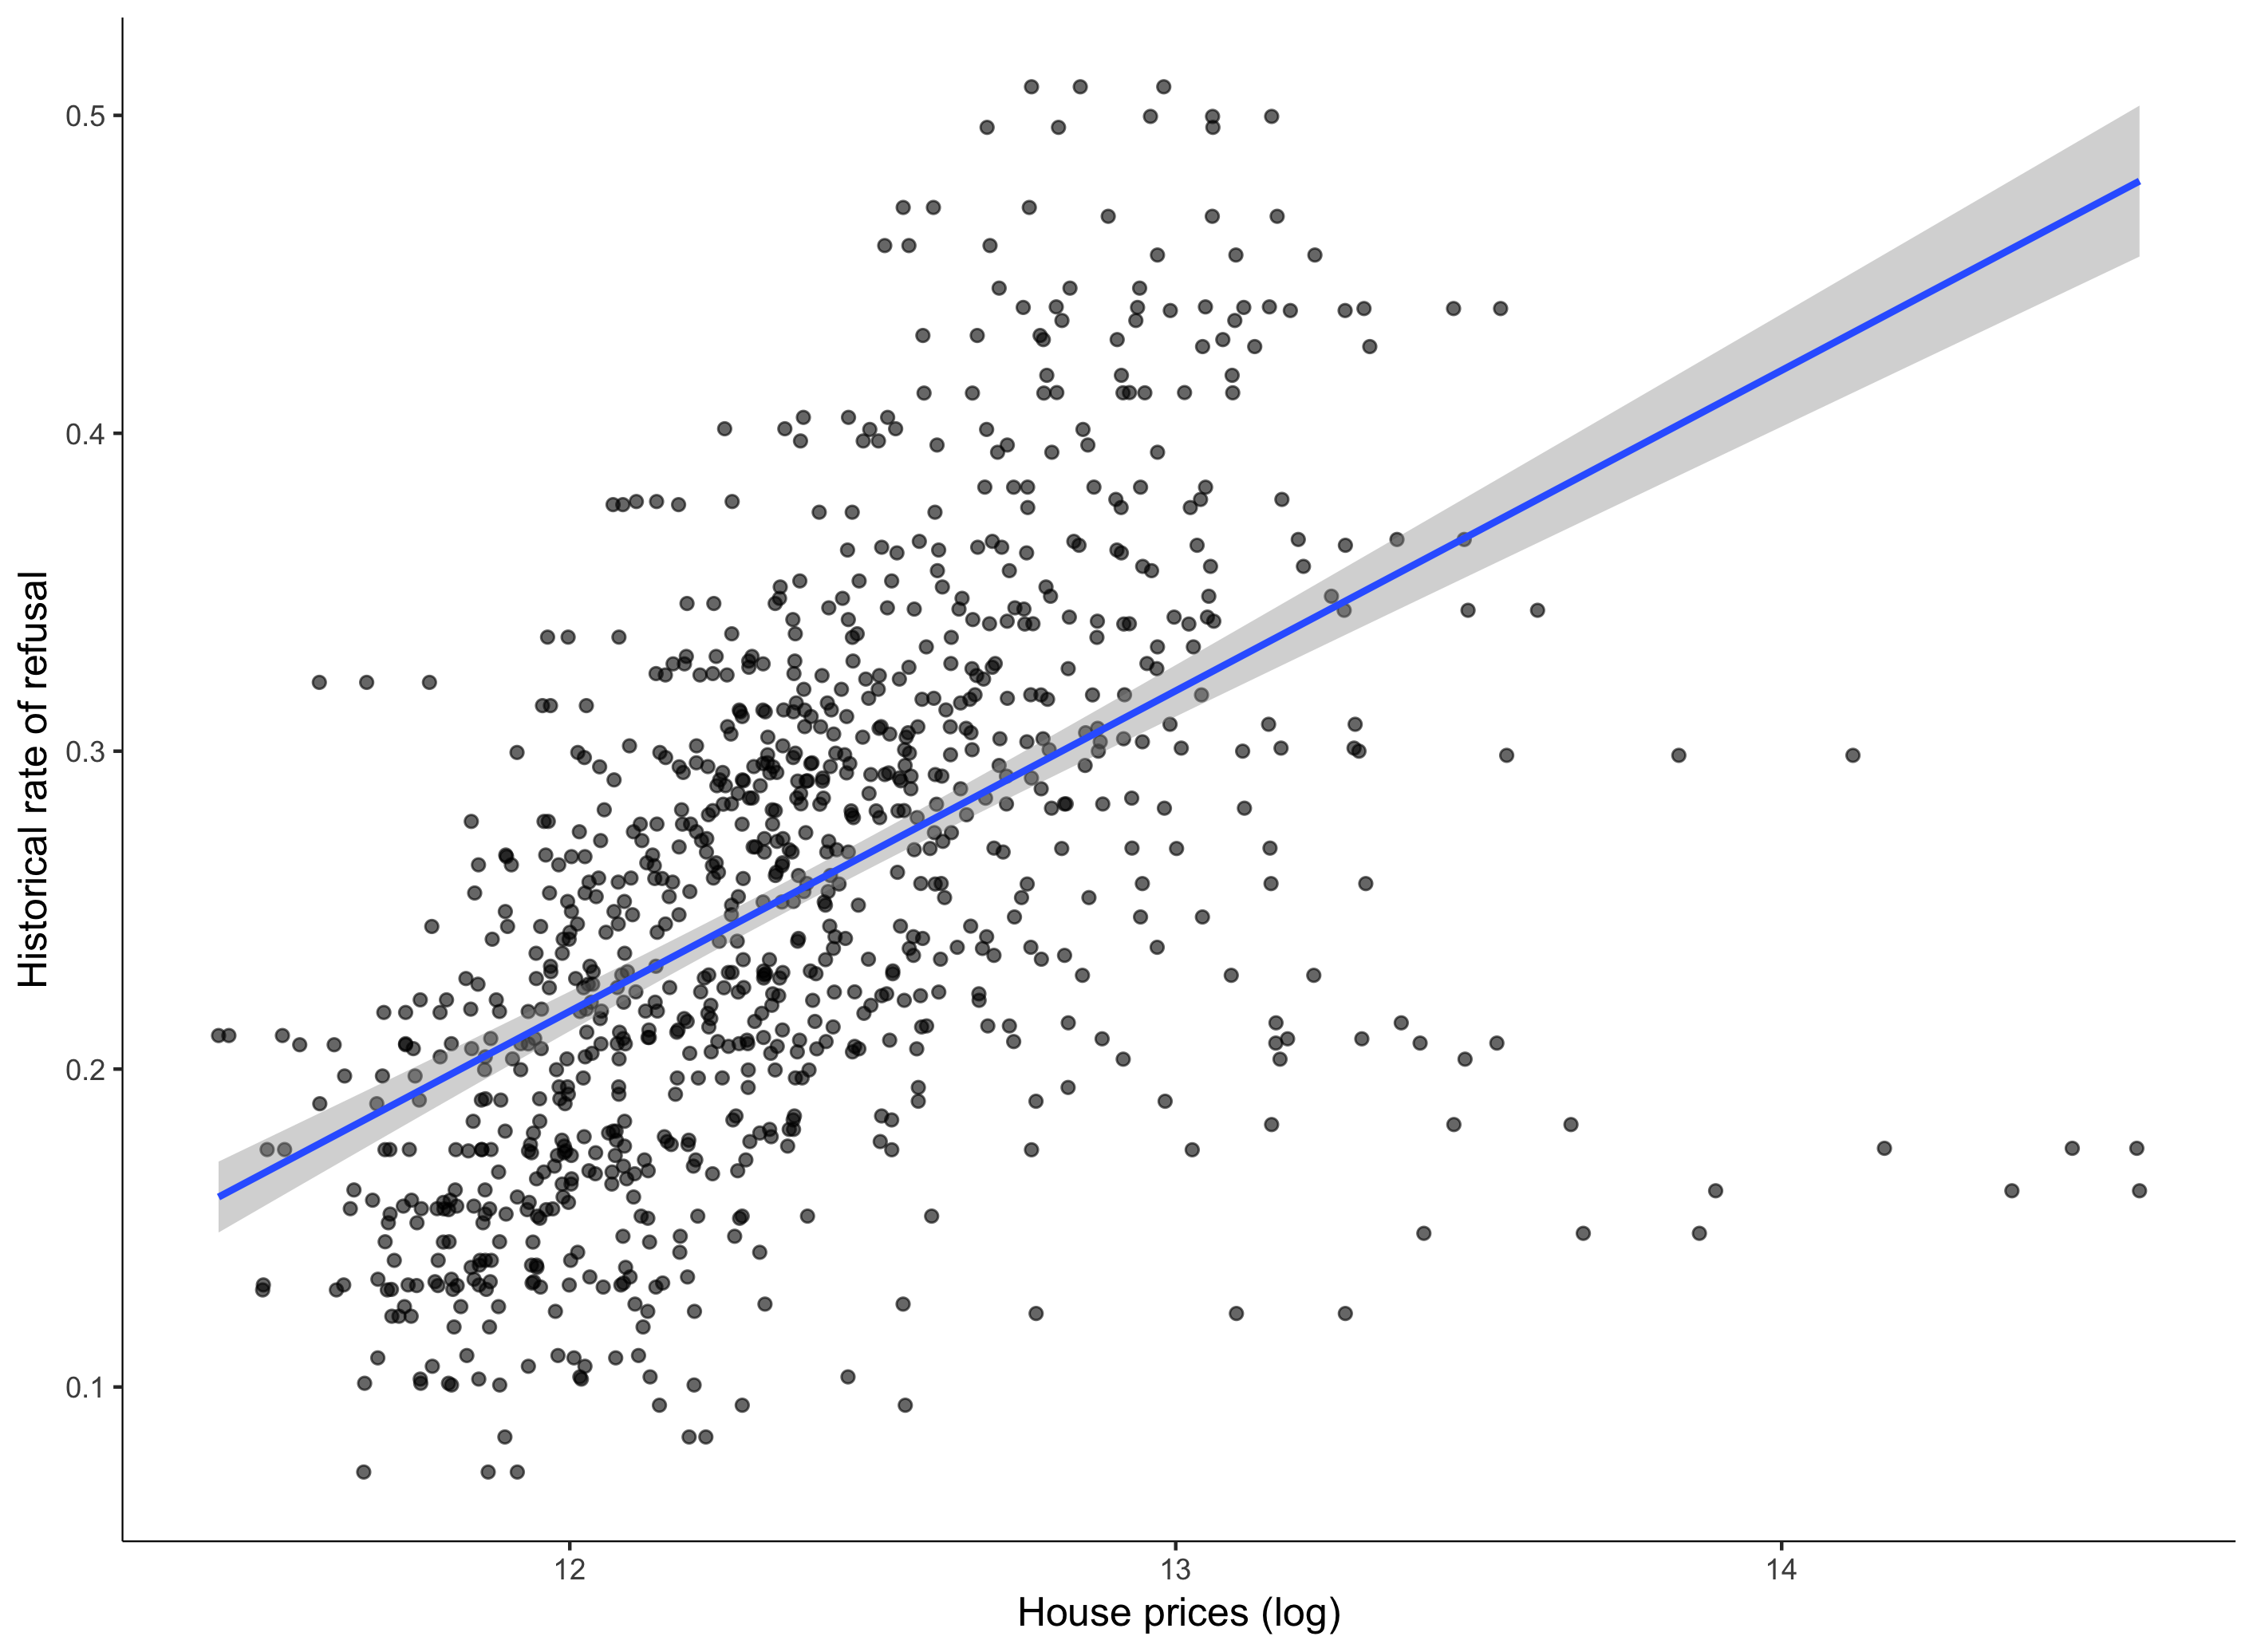
\includegraphics[width=1\textwidth]{corr_prices_refusal.png}
\caption{Correlation between urban planning restrictiveness and house prices}
\label{fig: corr_prices_refusal}
\end{figure}




\newpage

\begin{figure}[h!]
  
\begin{minipage}{\textwidth}
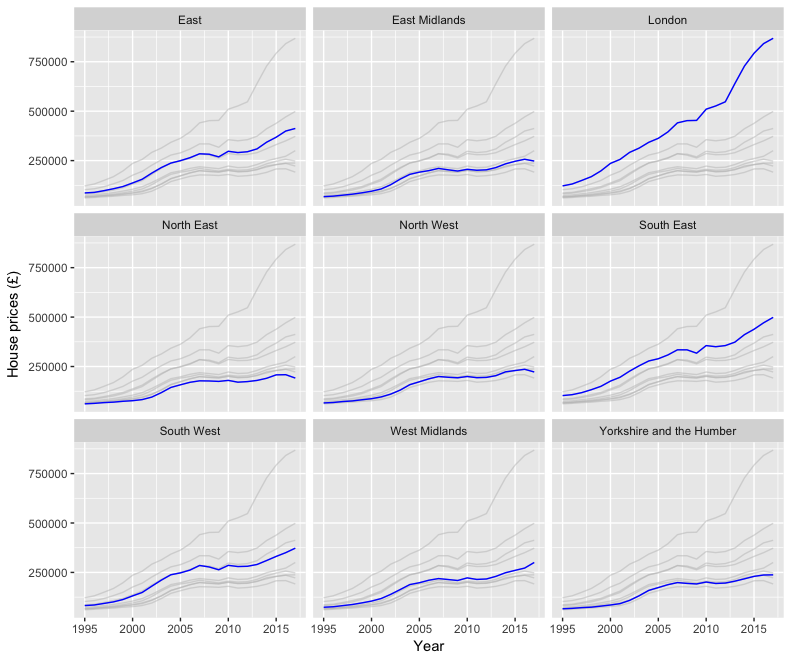
\includegraphics[width=1\textwidth]{house_prices_england_deflated.png}
\begin{flushright}
{\footnotesize Source: Office of National Statistics. House prices are deflated to 2000 prices.\par}
\end{flushright}
\end{minipage}
\caption{House prices in England, 1995-2017}
\label{fig: house_prices}
\end{figure}

\newpage


\begin{figure}[ht]
  \begin{minipage}{\textwidth}
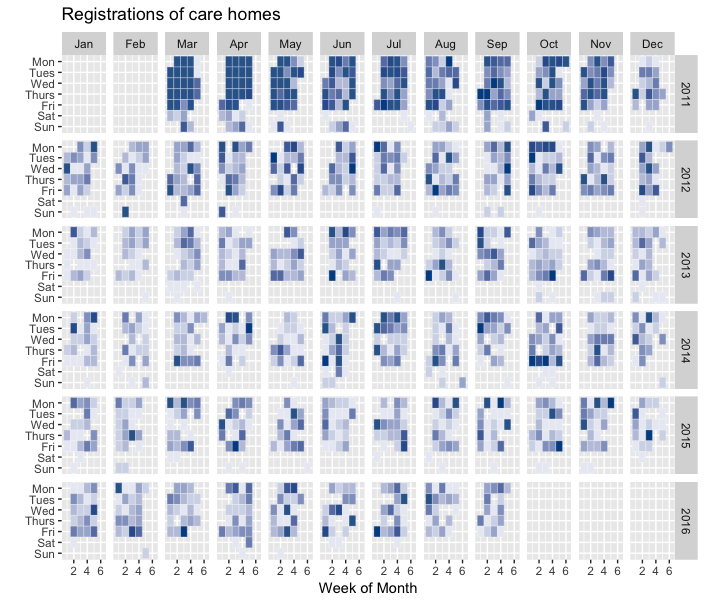
\includegraphics[width=1\textwidth]{registrations.png}
\begin{flushright}
{\footnotesize Source: Care Quality Commission.\par}
\end{flushright}
\end{minipage}
\caption{Care homes registrations in the CQC (2011- 2016)}
\label{fig: registrations}
\end{figure}


\newpage

\begin{figure}[]
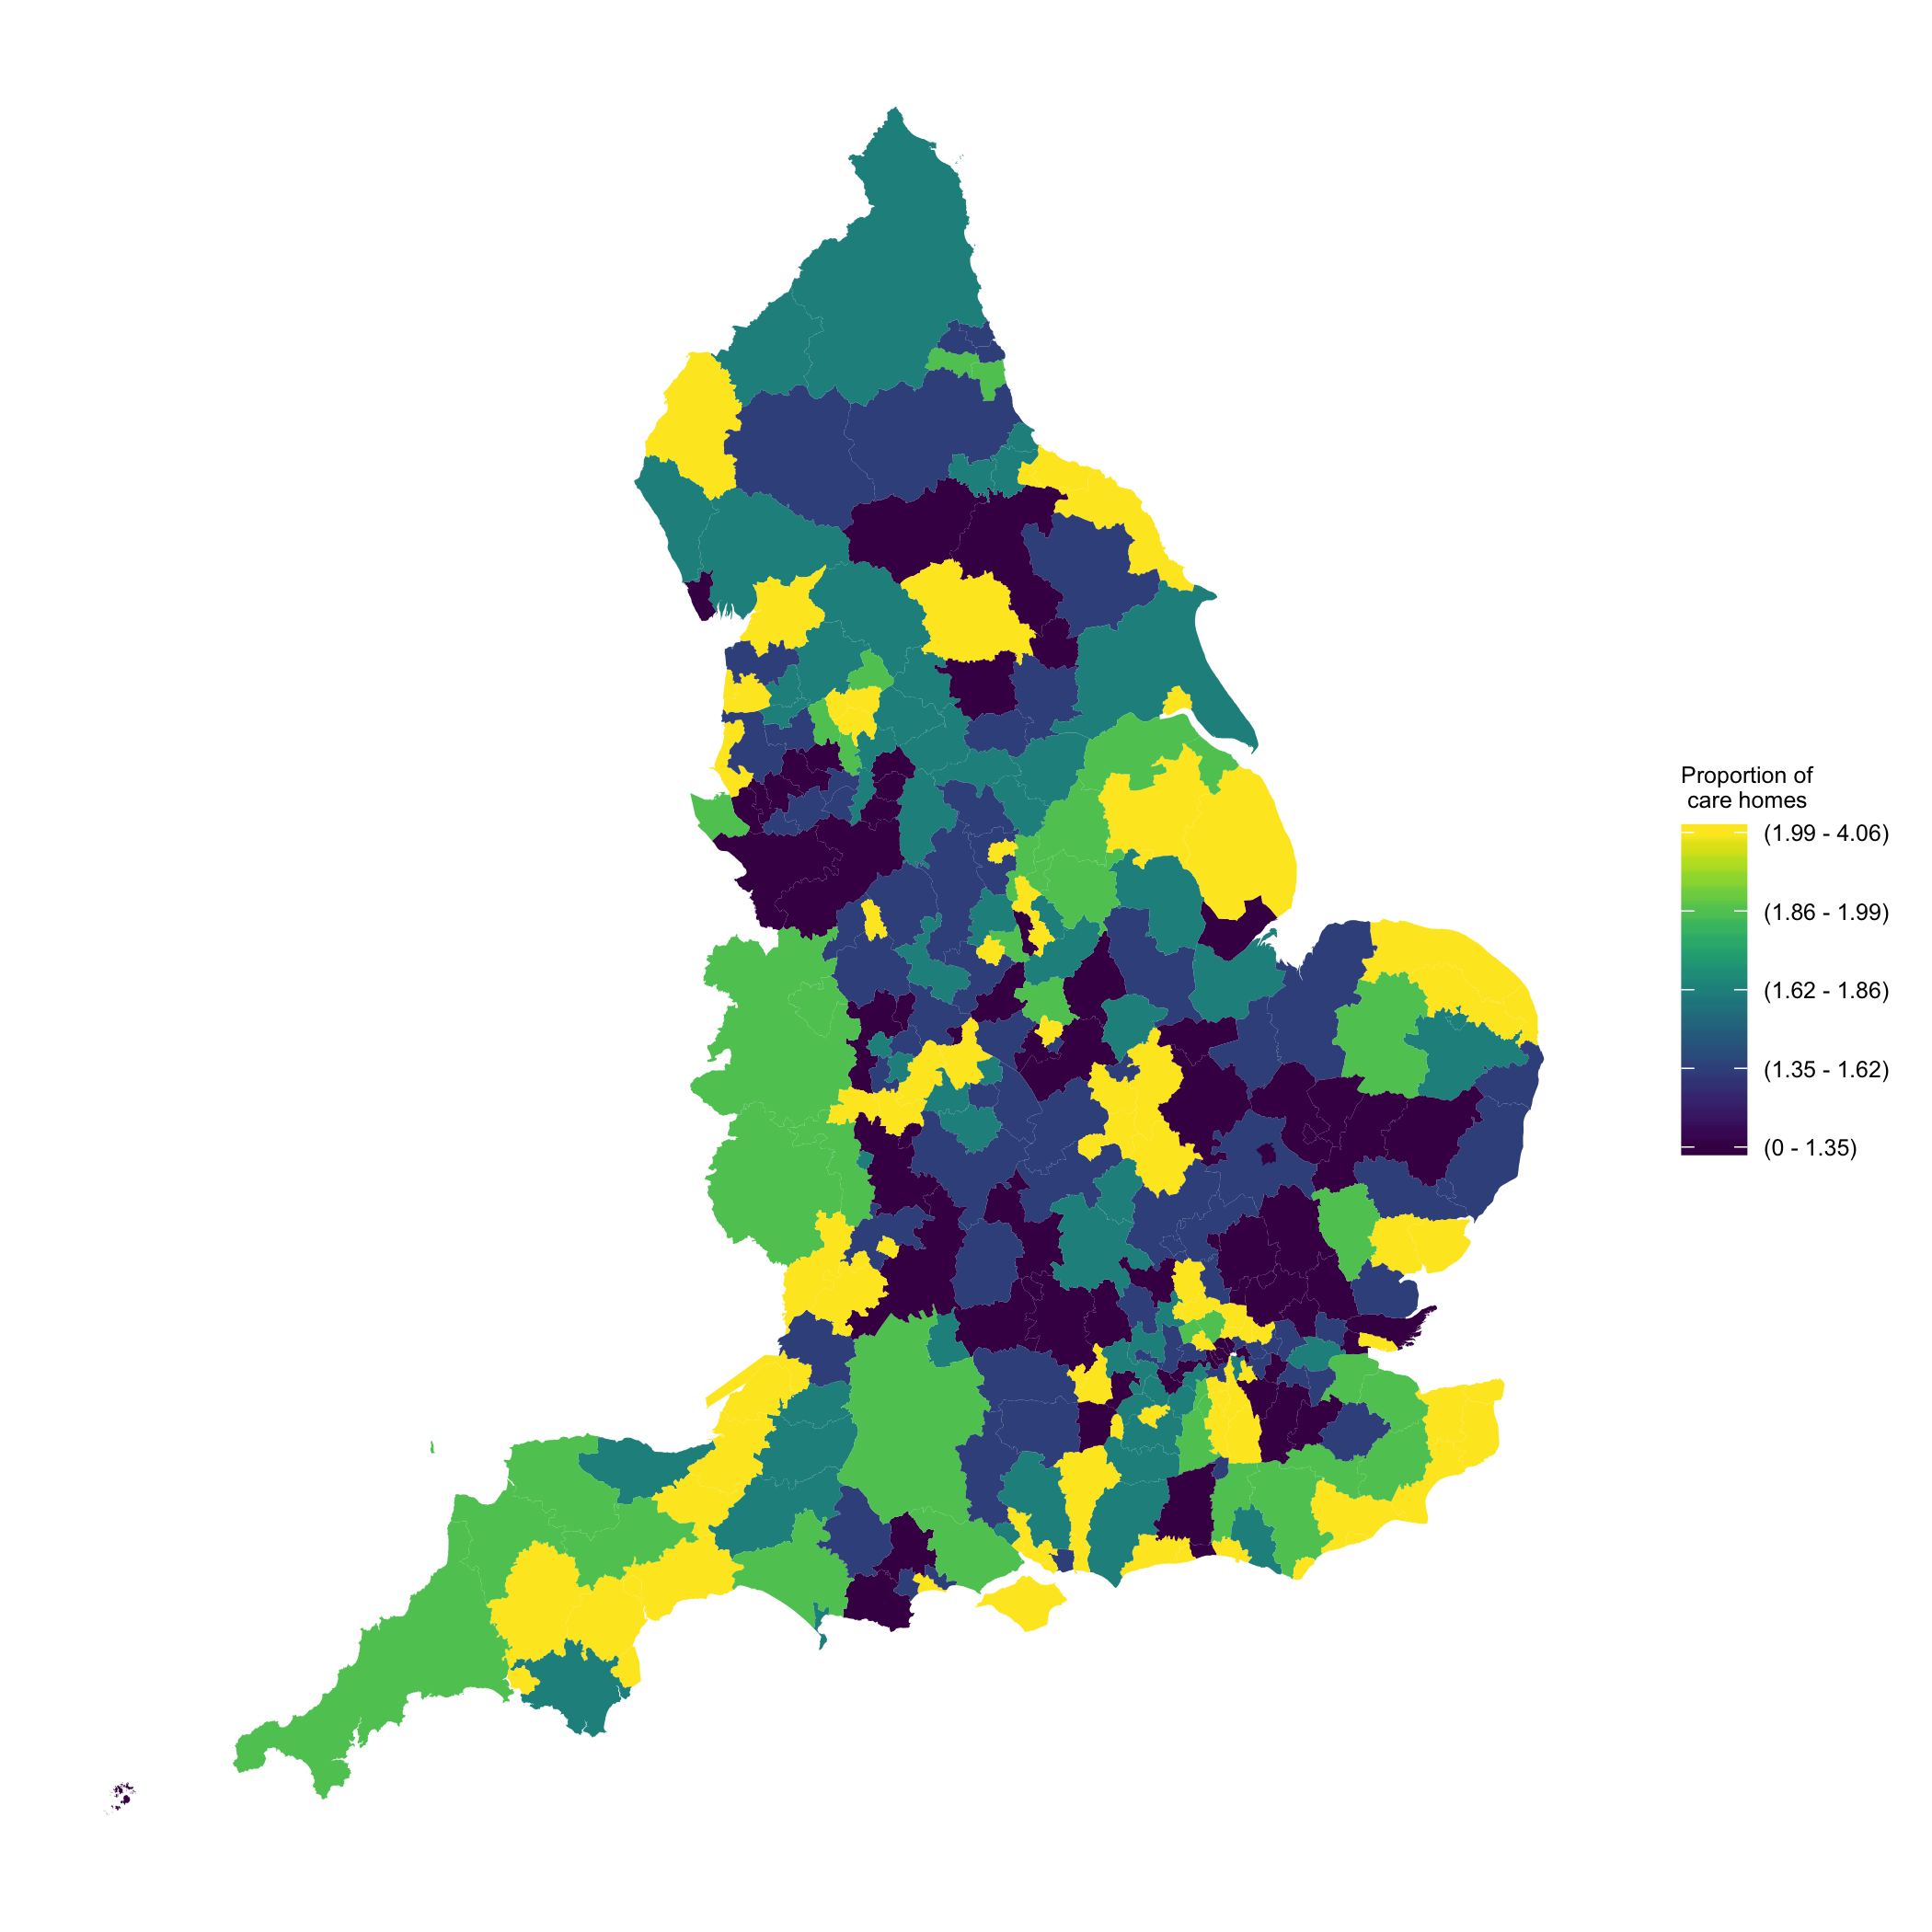
\includegraphics[width=1\textwidth]{map_carehomes.png}
\caption{Care homes per 1000 population over 65 - England, district level}
\label{fig: map care homes}
\end{figure}

\newpage

\begin{figure}[]
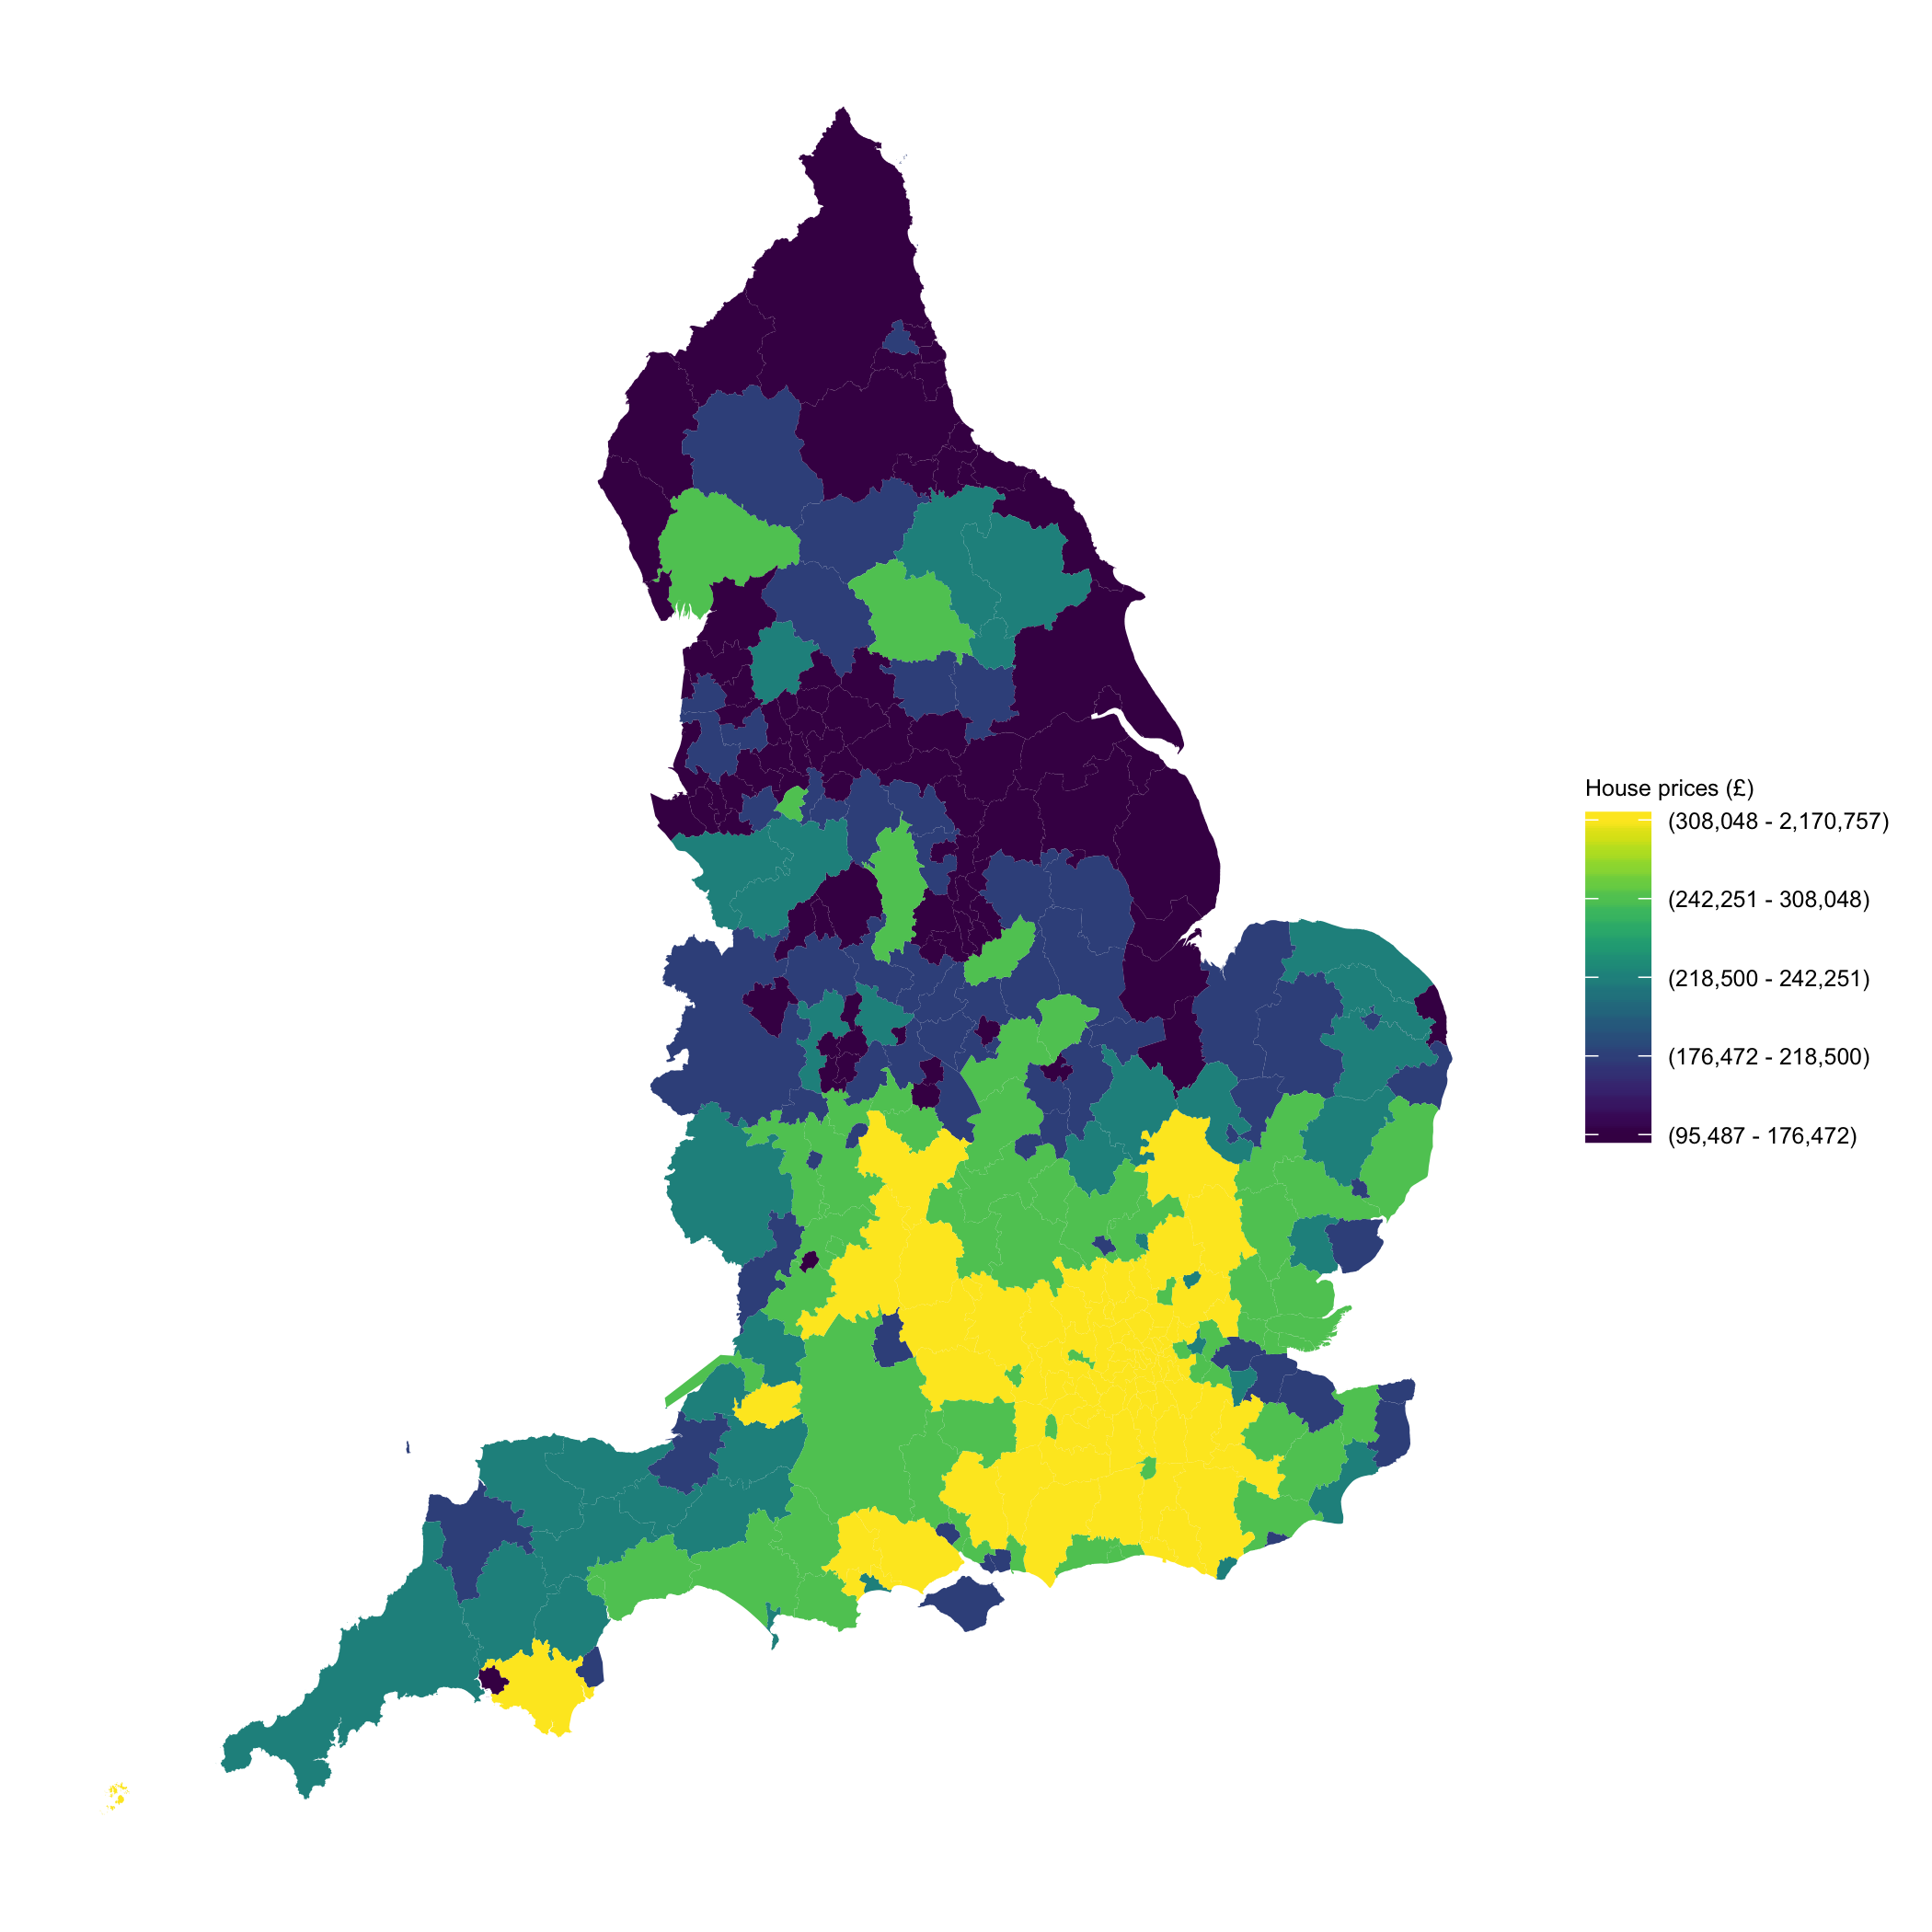
\includegraphics[width=1\textwidth]{map_price.png}
\caption{House prices - England, district level}
\label{fig: map house price}
\end{figure}




\newpage

\begin{figure}[h!]
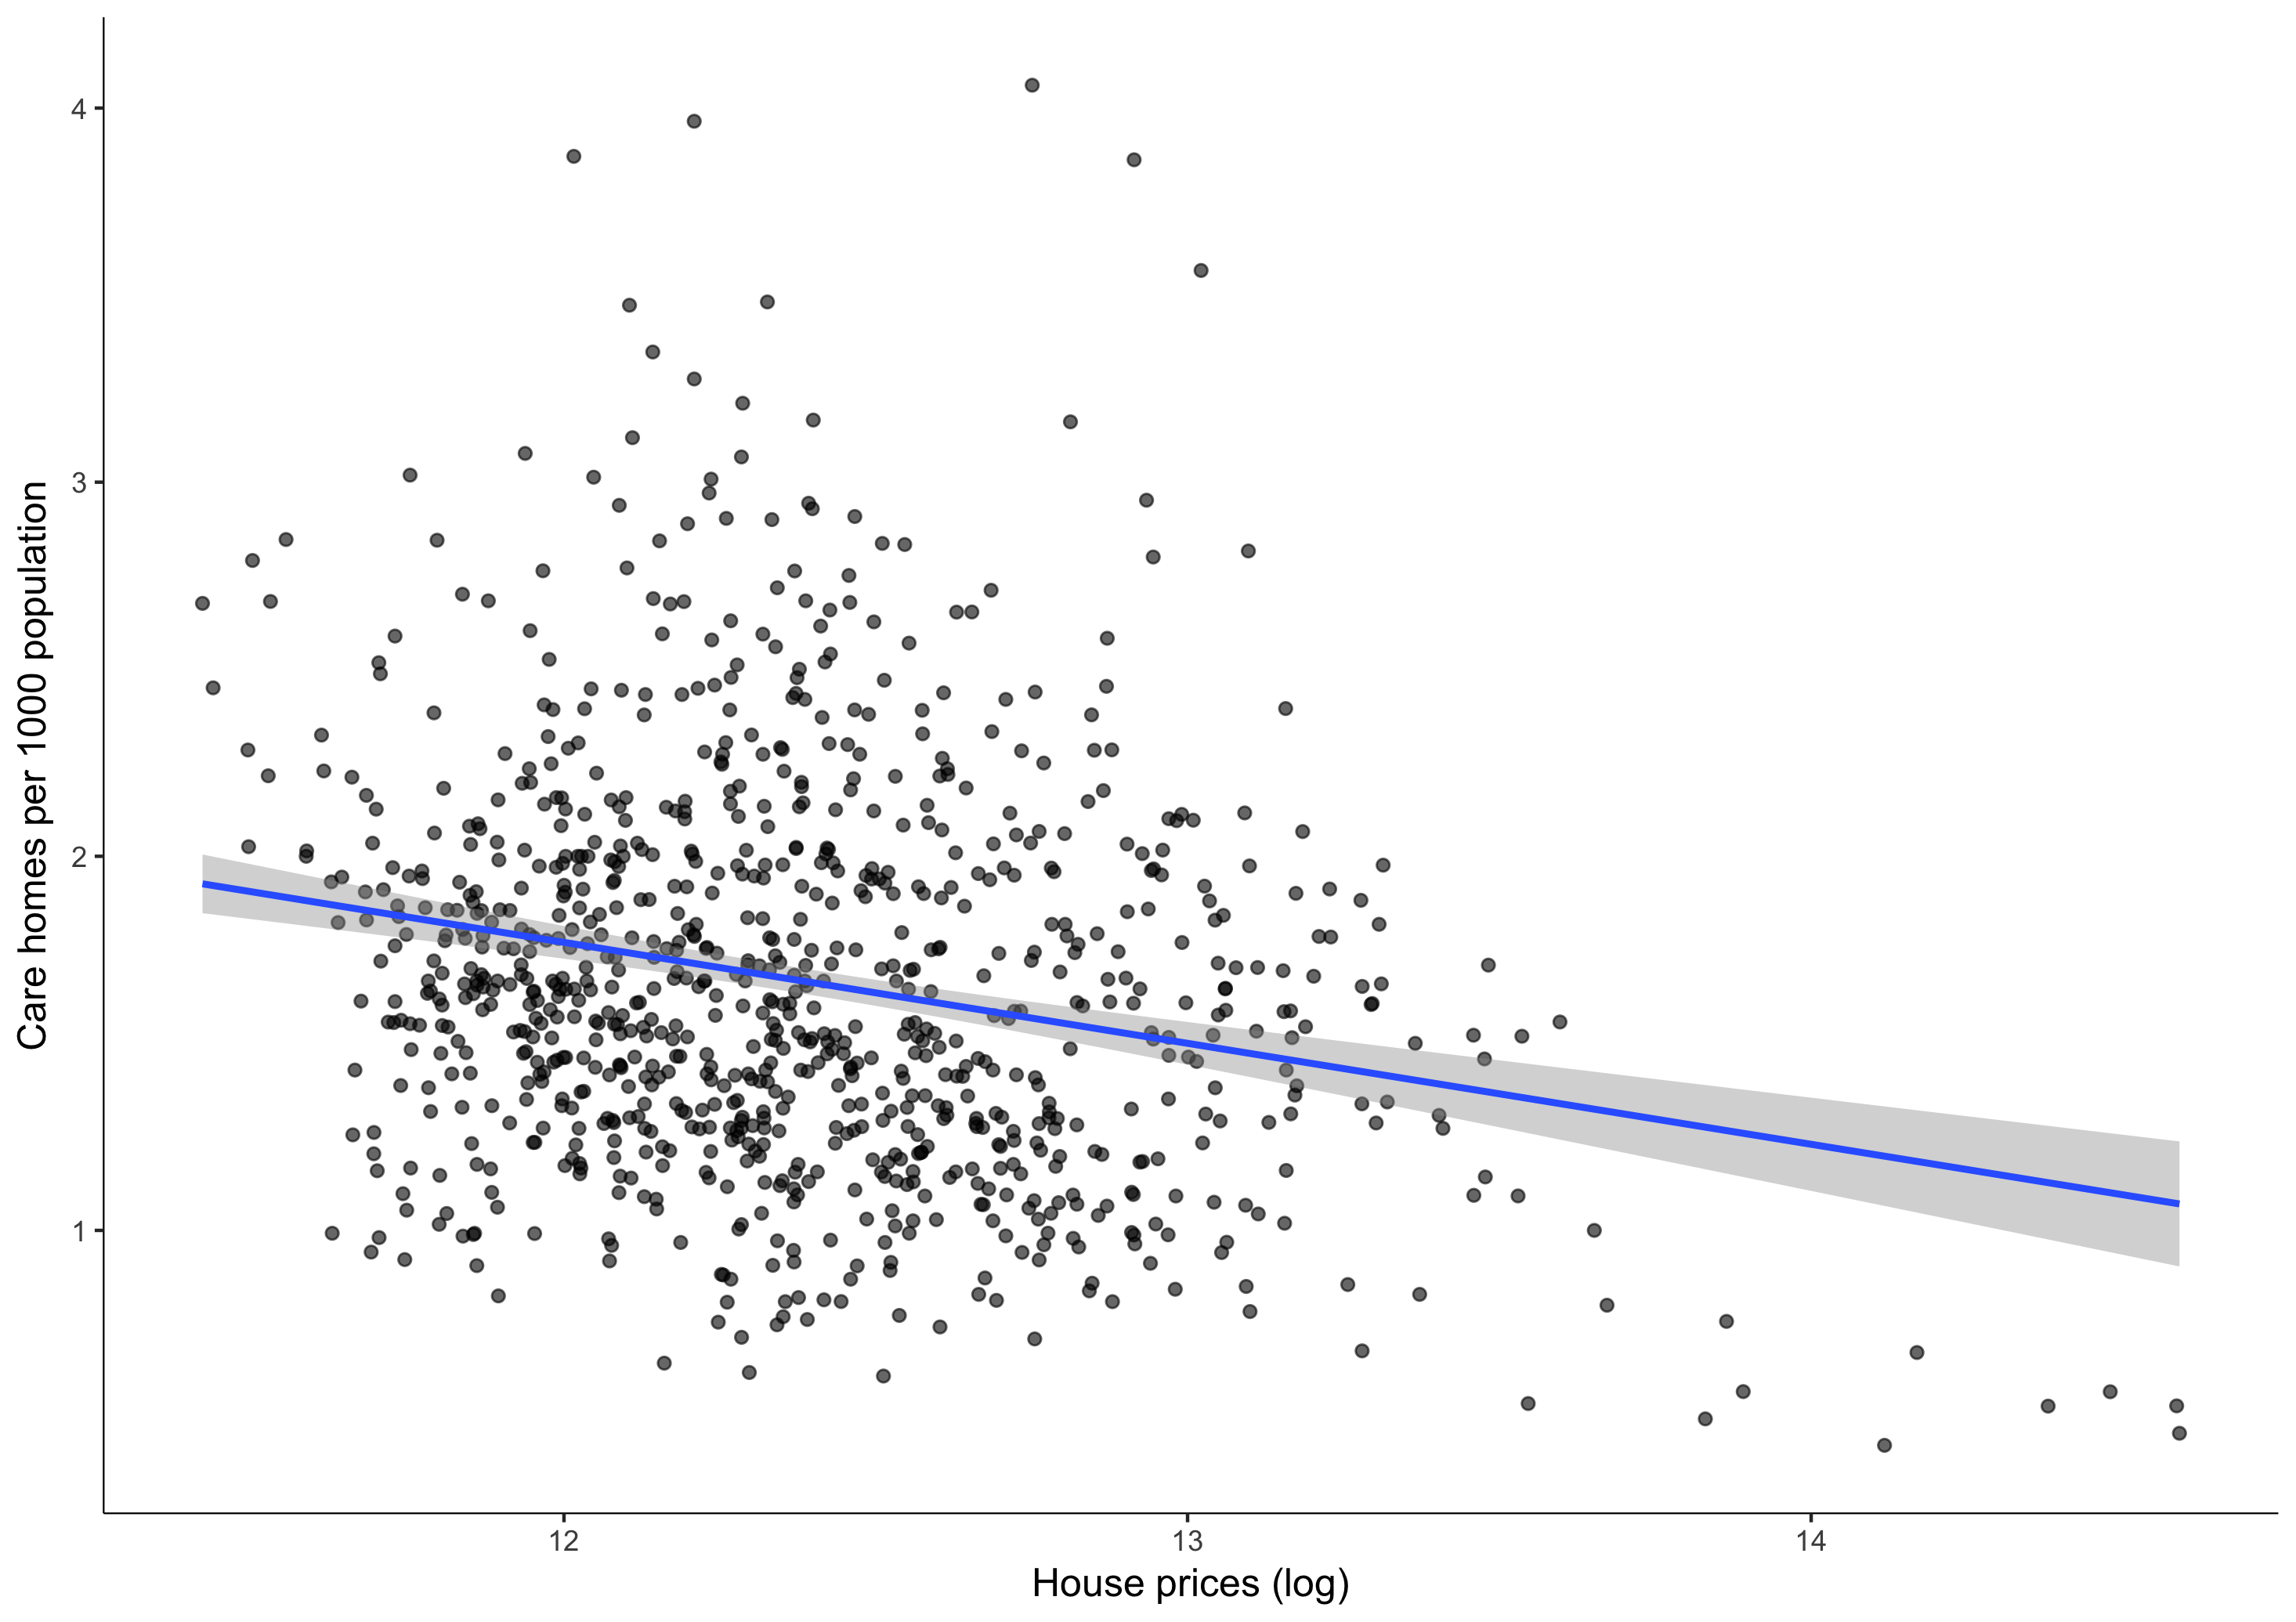
\includegraphics[width=1\textwidth]{corr_prices_carehomes.png}
\caption{Correlation between care homes and house prices}
\label{fig: carehomes_prices}
\end{figure}


\newpage

\begin{figure}[h!]
\begin{minipage}[t]{0.5\linewidth}
    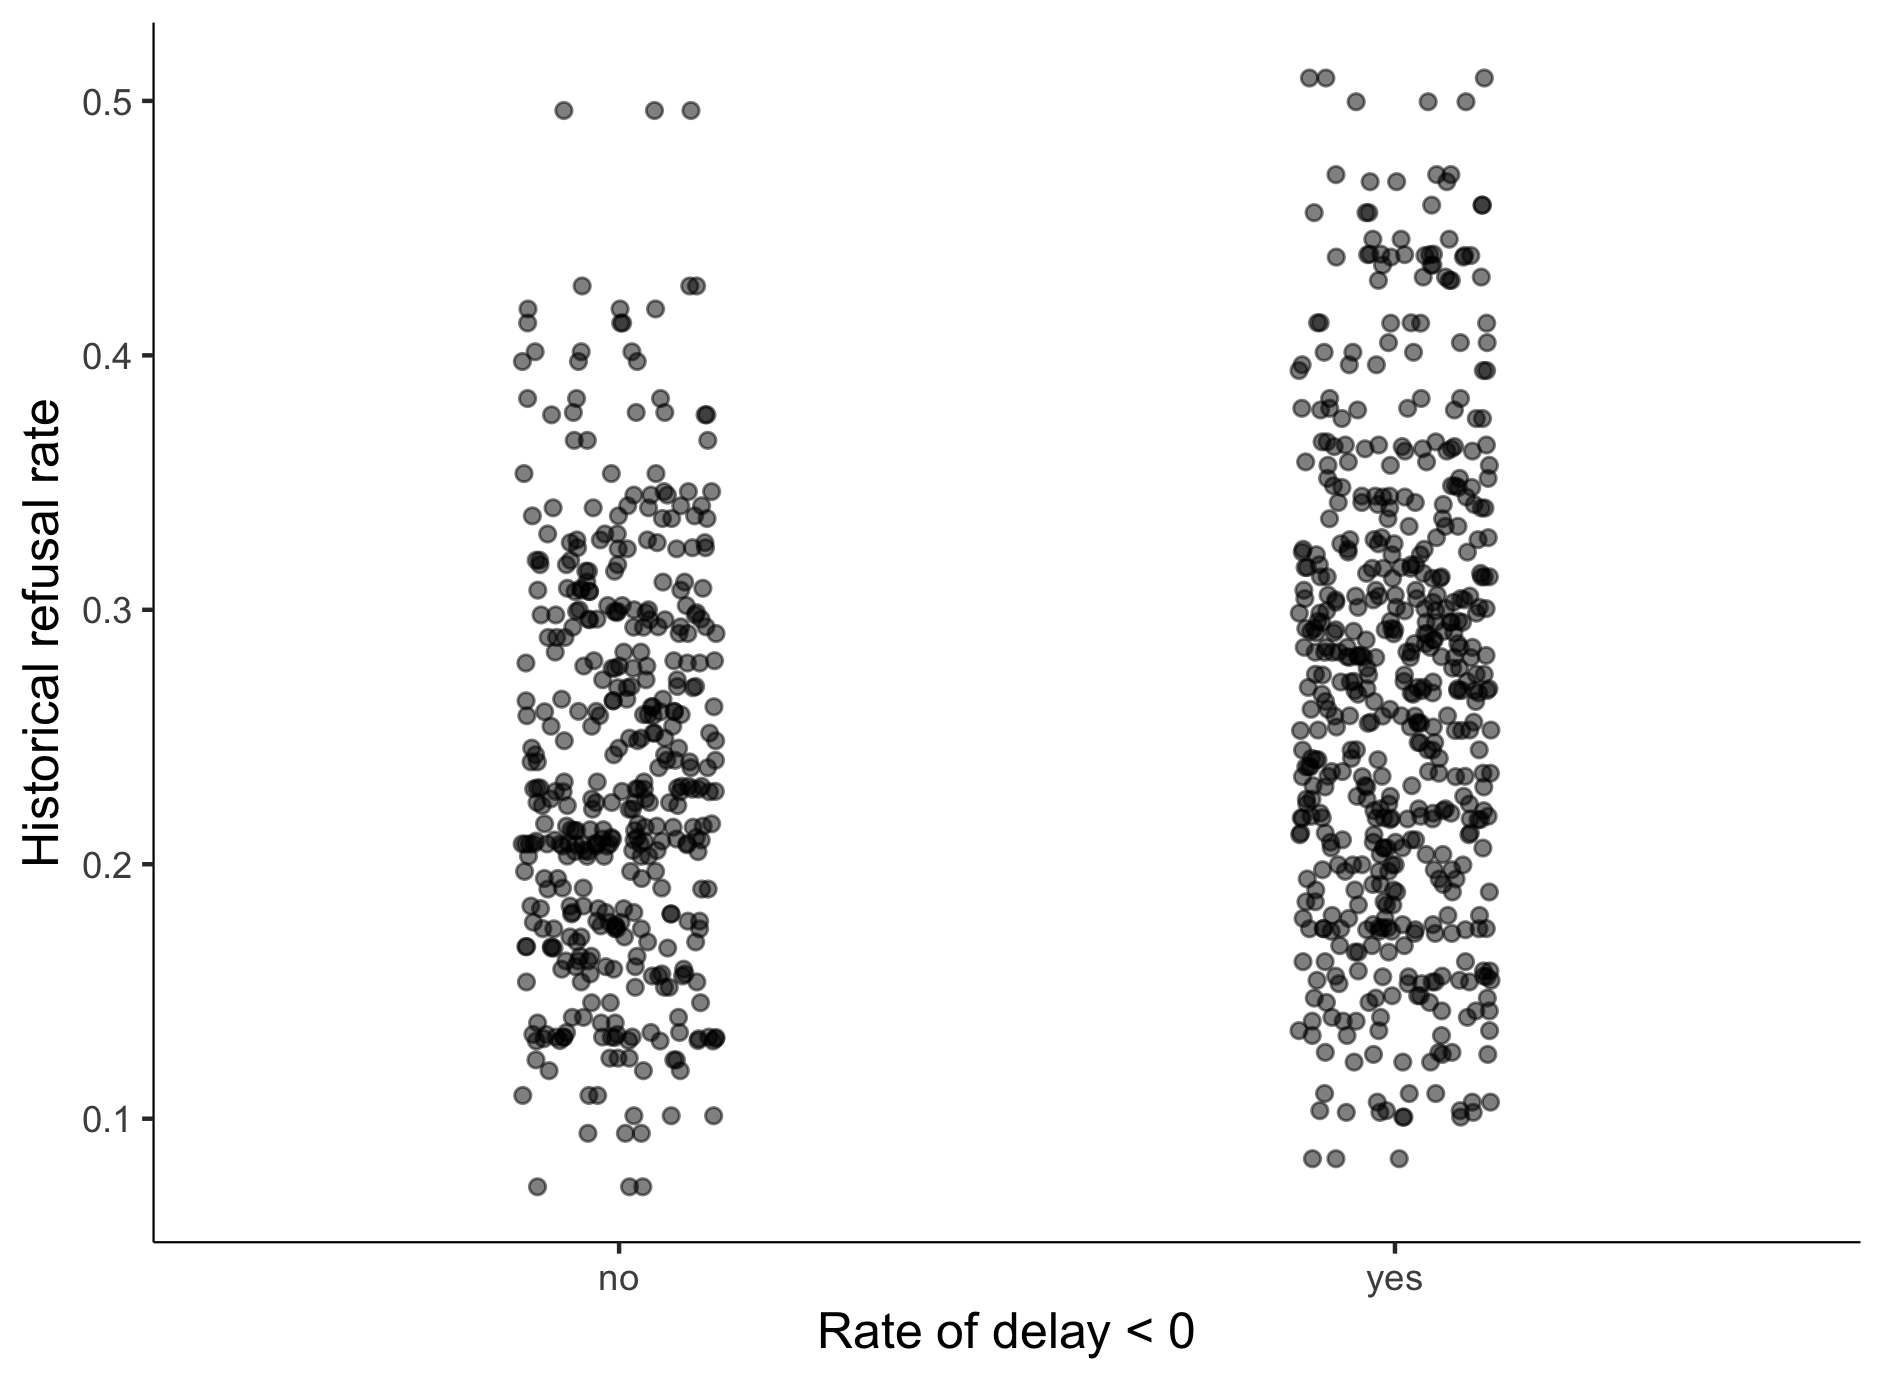
\includegraphics[width=\linewidth]{refusal.png}
    \caption{Historical refusal rate }
    \label{refusal_restrictive}
\end{minipage}%
%    \hfill%
\begin{minipage}[t]{0.45\linewidth}
    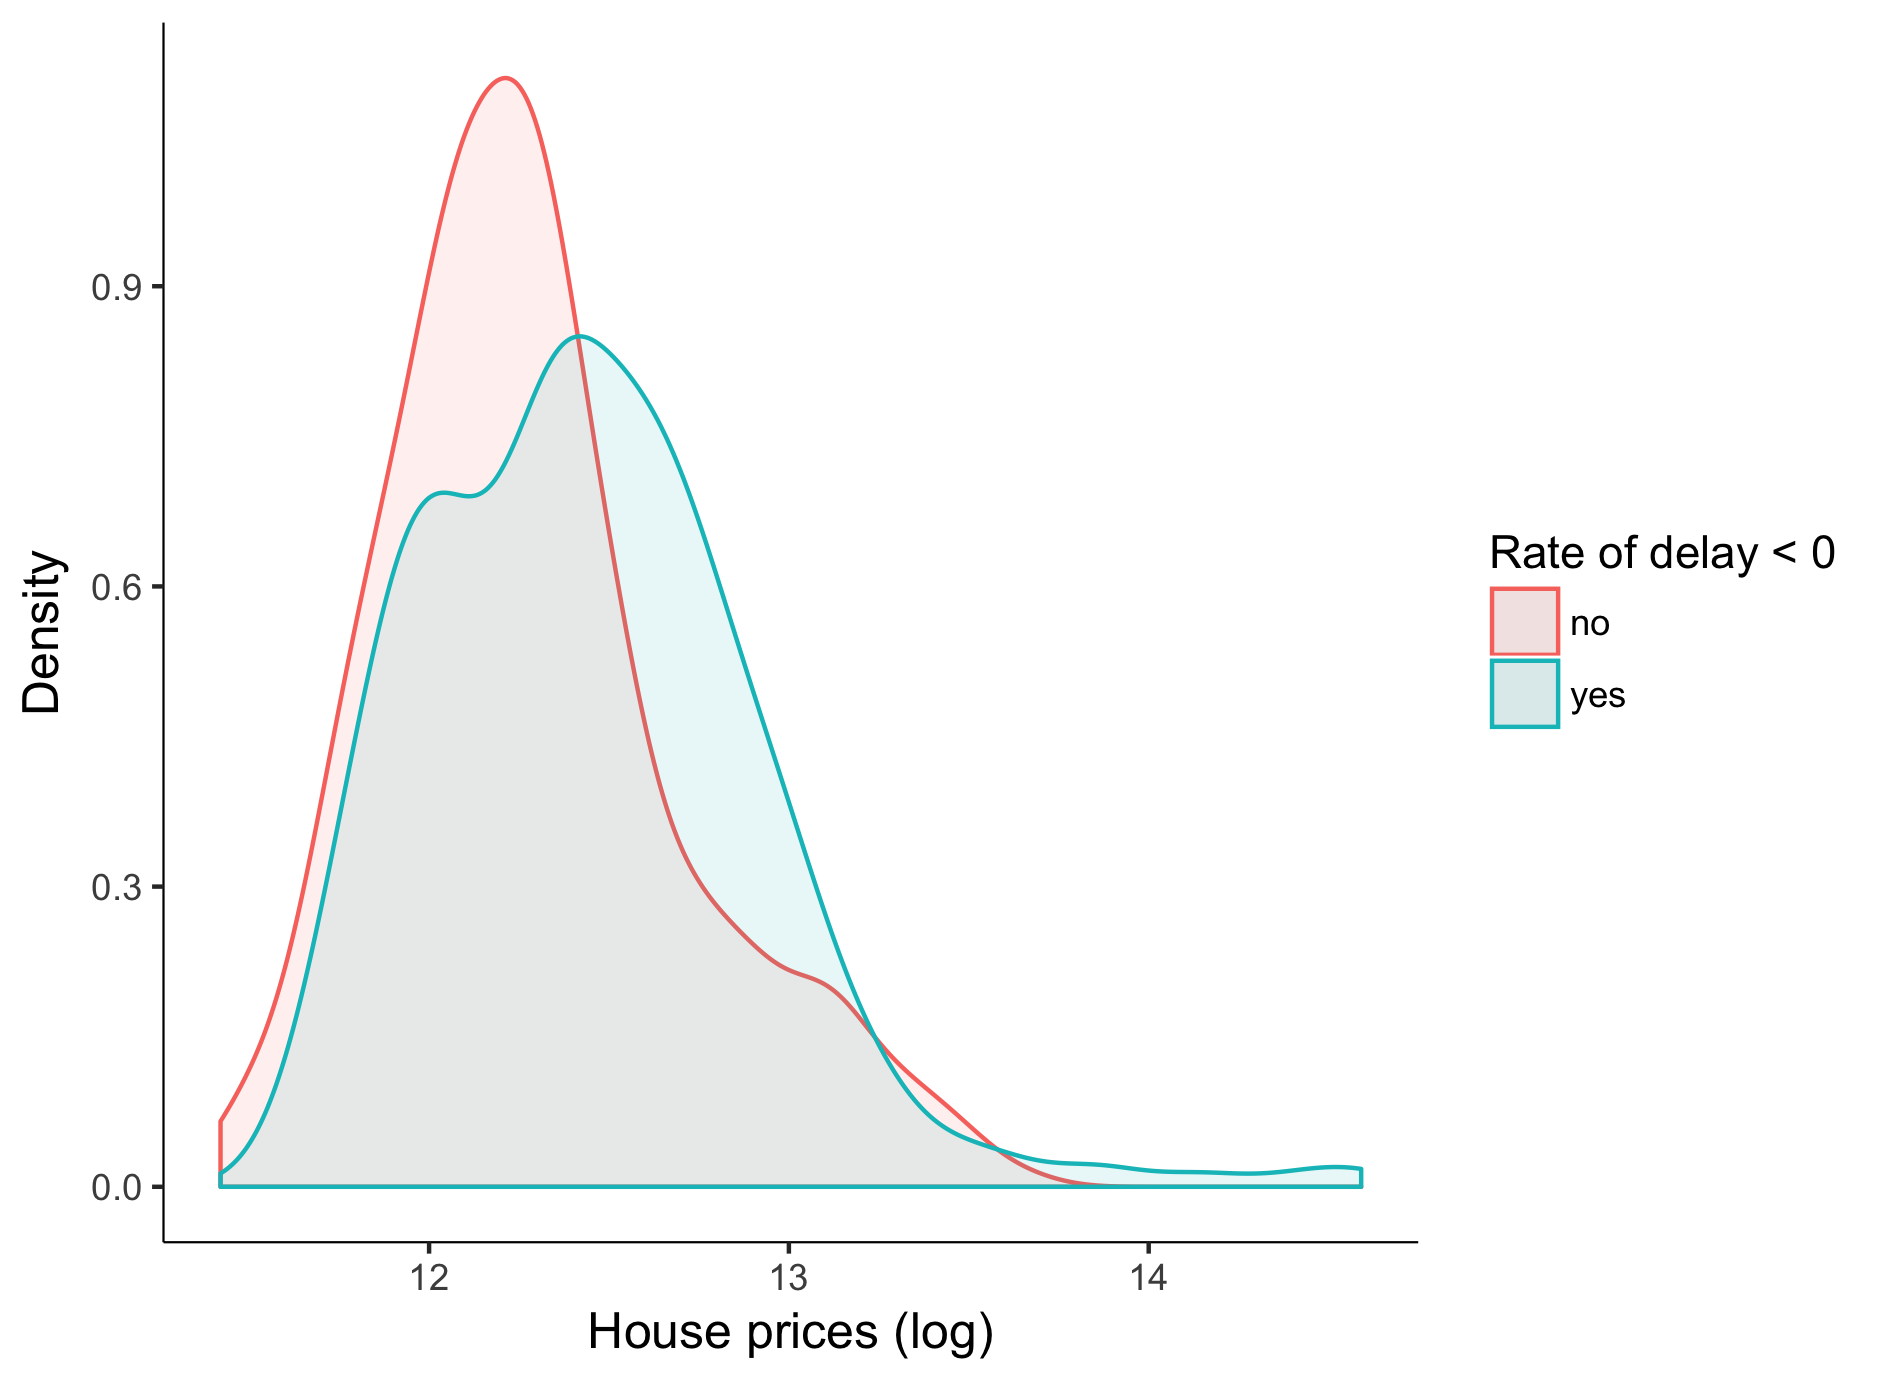
\includegraphics[width=\linewidth]{dens_complete.png}
    \caption{Distribution of house prices}
    \label{f2}
\end{minipage} 
\end{figure}


\newpage



\end{document}
